\chapter{Introduction}
\label{chap:1}

Palula [phl] is an~Indo"=Aryan language belonging to a~group of speech varieties subsumed under the heading
Shina. It is spoken by approximately 10,000 people in the Chitral Valley in northern Pakistan's
mountain region. This study is the first attempt at a~systematic description of the grammar of
a~language that, until recently, has been unwritten and largely undocumented. It is based on first
hand data, collected and analysed in close collaboration with Palula"=speaking language consultants
(specially acknowledged in \sectref{sec:1-6}), mainly during the period 1998--2008. The two main
dialects, both represented in this work, correspond to the main distribution of the speakers into
the two side valleys Ashret and Biori, with the geographical coordinates 35° 26′ 6″ N 71° 44′ 41″ E and 35° 28′ 24″ N 71° 48′ 2″ E, respectively.\footnote{The coordinates provided are those corresponding to the most densely populated section of each of the two main settlements, Atshareet"=xaás and Bhiúuṛi.}

\section{Language name}
\label{sec:1-1}

\textit{Palula} and \textit{Phalura} are the names most commonly used in linguistic and other
literature with reference to this speech variety, the former almost exclusively used in more recent
publications \citep{cacopardo2001,bashir2003,heegardpetersen2006,schmidtkohistani2008,perder2013,baart2014}. In the earliest reference in print to this particular ethnolinguistic group
\citep[64]{biddulph1986}, the ethnonym \textit{Dangariké} is used, but only a~few years later,
a~British officer named Gurdon, stationed in Chitral between 1895 and 1902, mentions that people in
some villages in southern Chitral speak a~language called \textit{Palola}, or
\textit{Dangarikwar}\footnote{The derivational suffix\textit{-war} denotes 'language' in Khowar, the
  \textit{lingua franca} of Chitral.} \citep{morgenstierne1941}.


Despite mainly using the name \textit{Palula} in his earlier references
(e.g., \citeyear[54--59]{morgenstierne1932}), the Norwegian linguist Georg Morgenstierne who conducted
field research in the region in the 1920s \citep{morgenstiernelorentzen1992} was the one who introduced the form \textit{Phalûṛa}
(\textit{Phalura} without diacritics), which is how the language was referred to in what was to
remain the sole source of scholarly knowledge about this language for decades
\citep{morgenstierne1941} and set a~standard followed by others
(\citealt{buddruss1967,edelman1983,masica1991,decker1992a}). It seems likely,
however, that this form was misconstrued, as there is no other primary source supporting it and no
recollection of it in the present"=day community of Palula speakers. The name \textit{Palula} was brought to the fore again by Richard~\citet{strand1997/2015}, based on
his own field studies (of the Ashret dialect) in the 1980s and was transcribed as \textit{palôlâ'}, although he himself primarily
refers to the language as \textit{açharêtâ'} (appr. `the speech of Ashret').


\textit{Palula} corresponds to the self"=designation \textit{paalúula} `Palula people'
(sg. \textit{paalúulu} `a male person of the Palula') and \textit{paaluulaá} `the language
of the Palula', both represented orthographically as ``Palula''. There is, however, no complete
internal consensus on what name to use for the language, one reason being that many speakers prefer
to identify their language as well as themselves with a~geographical location (a village or
a~valley), so that, for instance, the people of the Ashret Valley more readily refer to their tongue
as \textit{atshareetaá} (in my transcription corresponding to Strand's
açharêtâ'), as observed already by \citet{morgenstierne1941}, or the even more
generic \textit{asíi čoolaá} `our speech'. While the name Palula is indeed recognised by
people with some historical awareness and a~certain educational level\footnote{This was reflected in
  the choice of a~name for the local language society formed in 2003 by representatives from all the
  major locations: \textit{Anjuman-e-Taraqqi-e-Palula}, approximately meaning `The Society for the Promotion of Palula'.} in both of the main geographical locations, it is also accepted at large by the speakers
in the Biori Valley as a~reference to their own speech as well as that of Ashret, whereas the common
man in the Ashret Valley tends to regard Palula as designating the (slightly different) speech
variety of the Biori Valley, often implying an~additional ``tribal''\footnote{While ``tribal'' in
  today's Western context is a~marked term in comparison to ``ethnic'', \textit{tribal} in the
  Pakistani context is on the contrary the politically correct choice as opposed to ethnic, the
  latter being avoided as carrying a~connotation of separatism; compare for instance with the fully accepted designations
  \textit{Federally Administered Tribal Areas} and \textit{Home and Tribal Affairs Department}.} and
genealogical distinction.

\largerpage
There are no suggestions as to the origin of the name Palula in the older literature, apart from \citeauthor{morgenstierne1941}'s (\citeyear[53]{morgenstierne1941}) comment that the name of the language (in its assumedly misapprehended form) is formally identical to the plural of `grain'. Recently however, the Italian anthropologist Alberto Cacopardo (\citeyear[91]{cacopardo2001}), has suggested a~historical link between the fifth- to eighth"=century Paṭola, or Palola, dynasty with its heart"=land in the upper Indus Valley and the ancestors of the Palula speakers, who according to local oral history, migrated from the very same area. The similarity between the names is, as \citet[3]{schmidtkohistani2008} point out, too striking to be merely coincidental.


In popular use by most outsiders~-- mainly speakers of Khowar (the linguistic majority of the district)~-- is the ethnonym \textit{Dangarik},
alternatively \textit{Dangeri} or \textit{Dangarikwar}, for the language itself. That use, however,
is frowned upon by many Palula speakers, particularly in the Ashret Valley. Following
\citet[113]{biddulph1986}, the term Dangariké was in the past applied to Shina"=speaking people in general, including the Chitrali Dangariké (i.e., the inhabitants of Ashret and Biori), carrying the
connotation ``cow"=people''. The same IA source lexeme \textit{ḍanɡara-}
\citep[5526, 5524]{turner1966} has given rise to derogatory meanings such as `defective, bad,
unpleasant' (see \citealt[81]{cacopardo2001} for a~discussion on this). In any case, the term has
often been, and is still, interpreted as derogatory by some (\citealt[69]{decker1992a};
\citeyear[160]{decker1996}, and own observations), and should therefore be avoided. A positive
explanation of the same word has, on the other hand, been offered to me by the local historian Muhammad Atiqullah from Biori as merely pointing to the geographical origin of the speech community in or near to
Tangir in the Indus Valley east of Chitral. It is of course not entirely unlikely that it is exactly
the use of wordplay itself that has given rise to the interpretational ambiguity, i.e., a~designation
intended to refer to geography being similar to a~derogatory word and is subsequently applied to
a~community already socially stigmatised or markedly different.


Finally, some of the more educated speakers of Palula would occasionally identify their language as a~dialect of Shina (\citealt[82]{decker1992a} and my own observations), although there is no evidence of any regular modern"=day interaction between Palula speakers in Chitral and speakers of any other Shina variety. 

\section{The general setting}
\label{sec:1-2}
\subsection{Where and by whom the language is spoken}
\label{subsec:1-2-1}

The geographical home of Palula is the southern part of Chitral district, in Pakistan's Khyber Pakhtunkhwa Province, displayed in Map~\ref{map:1-1}. All of the Palula speaking localities are
situated within a~stretch of only 40 kilometres on the eastern side of the Kunar River (also called
Chitral River), which crosses into neighbouring Afghanistan a~few kilometres down"=river from the
area where the language is spoken. The two main settlements of Palula speakers are the two side valleys Ashret and Biori. The main road, leading from lowland Pakistan to Chitral through the 10,000\,ft. Lowari Pass, goes right through the Ashret Valley. 


Although formally regarded as one large village, Ashret (Atshareét) is more accurately described as a~rather long stretch of more or less interconnected smaller villages or hamlets (coming from the Lowari Pass going downstream towards the main valley): Buzeeghaá, Bharaaḍám, Patoodhám, Lookúṛi, Kaṇeeghaá, Šaṛadeéš, Kooḍghaá, Ghróom (or Atshareet"=xaás `Ashret proper'), Feerimaá and Looṭanghaá. Apart from Buzeeghaá, which has a~majority of Pashto speakers, the population of all of these hamlets is solidly Palula"=speaking. The main settlement is situated at an altitude of 1,500 metres above sea level.

\begin{mapfigure}[p!]
\caption{The Palula"=speaking area in southern Chitral}
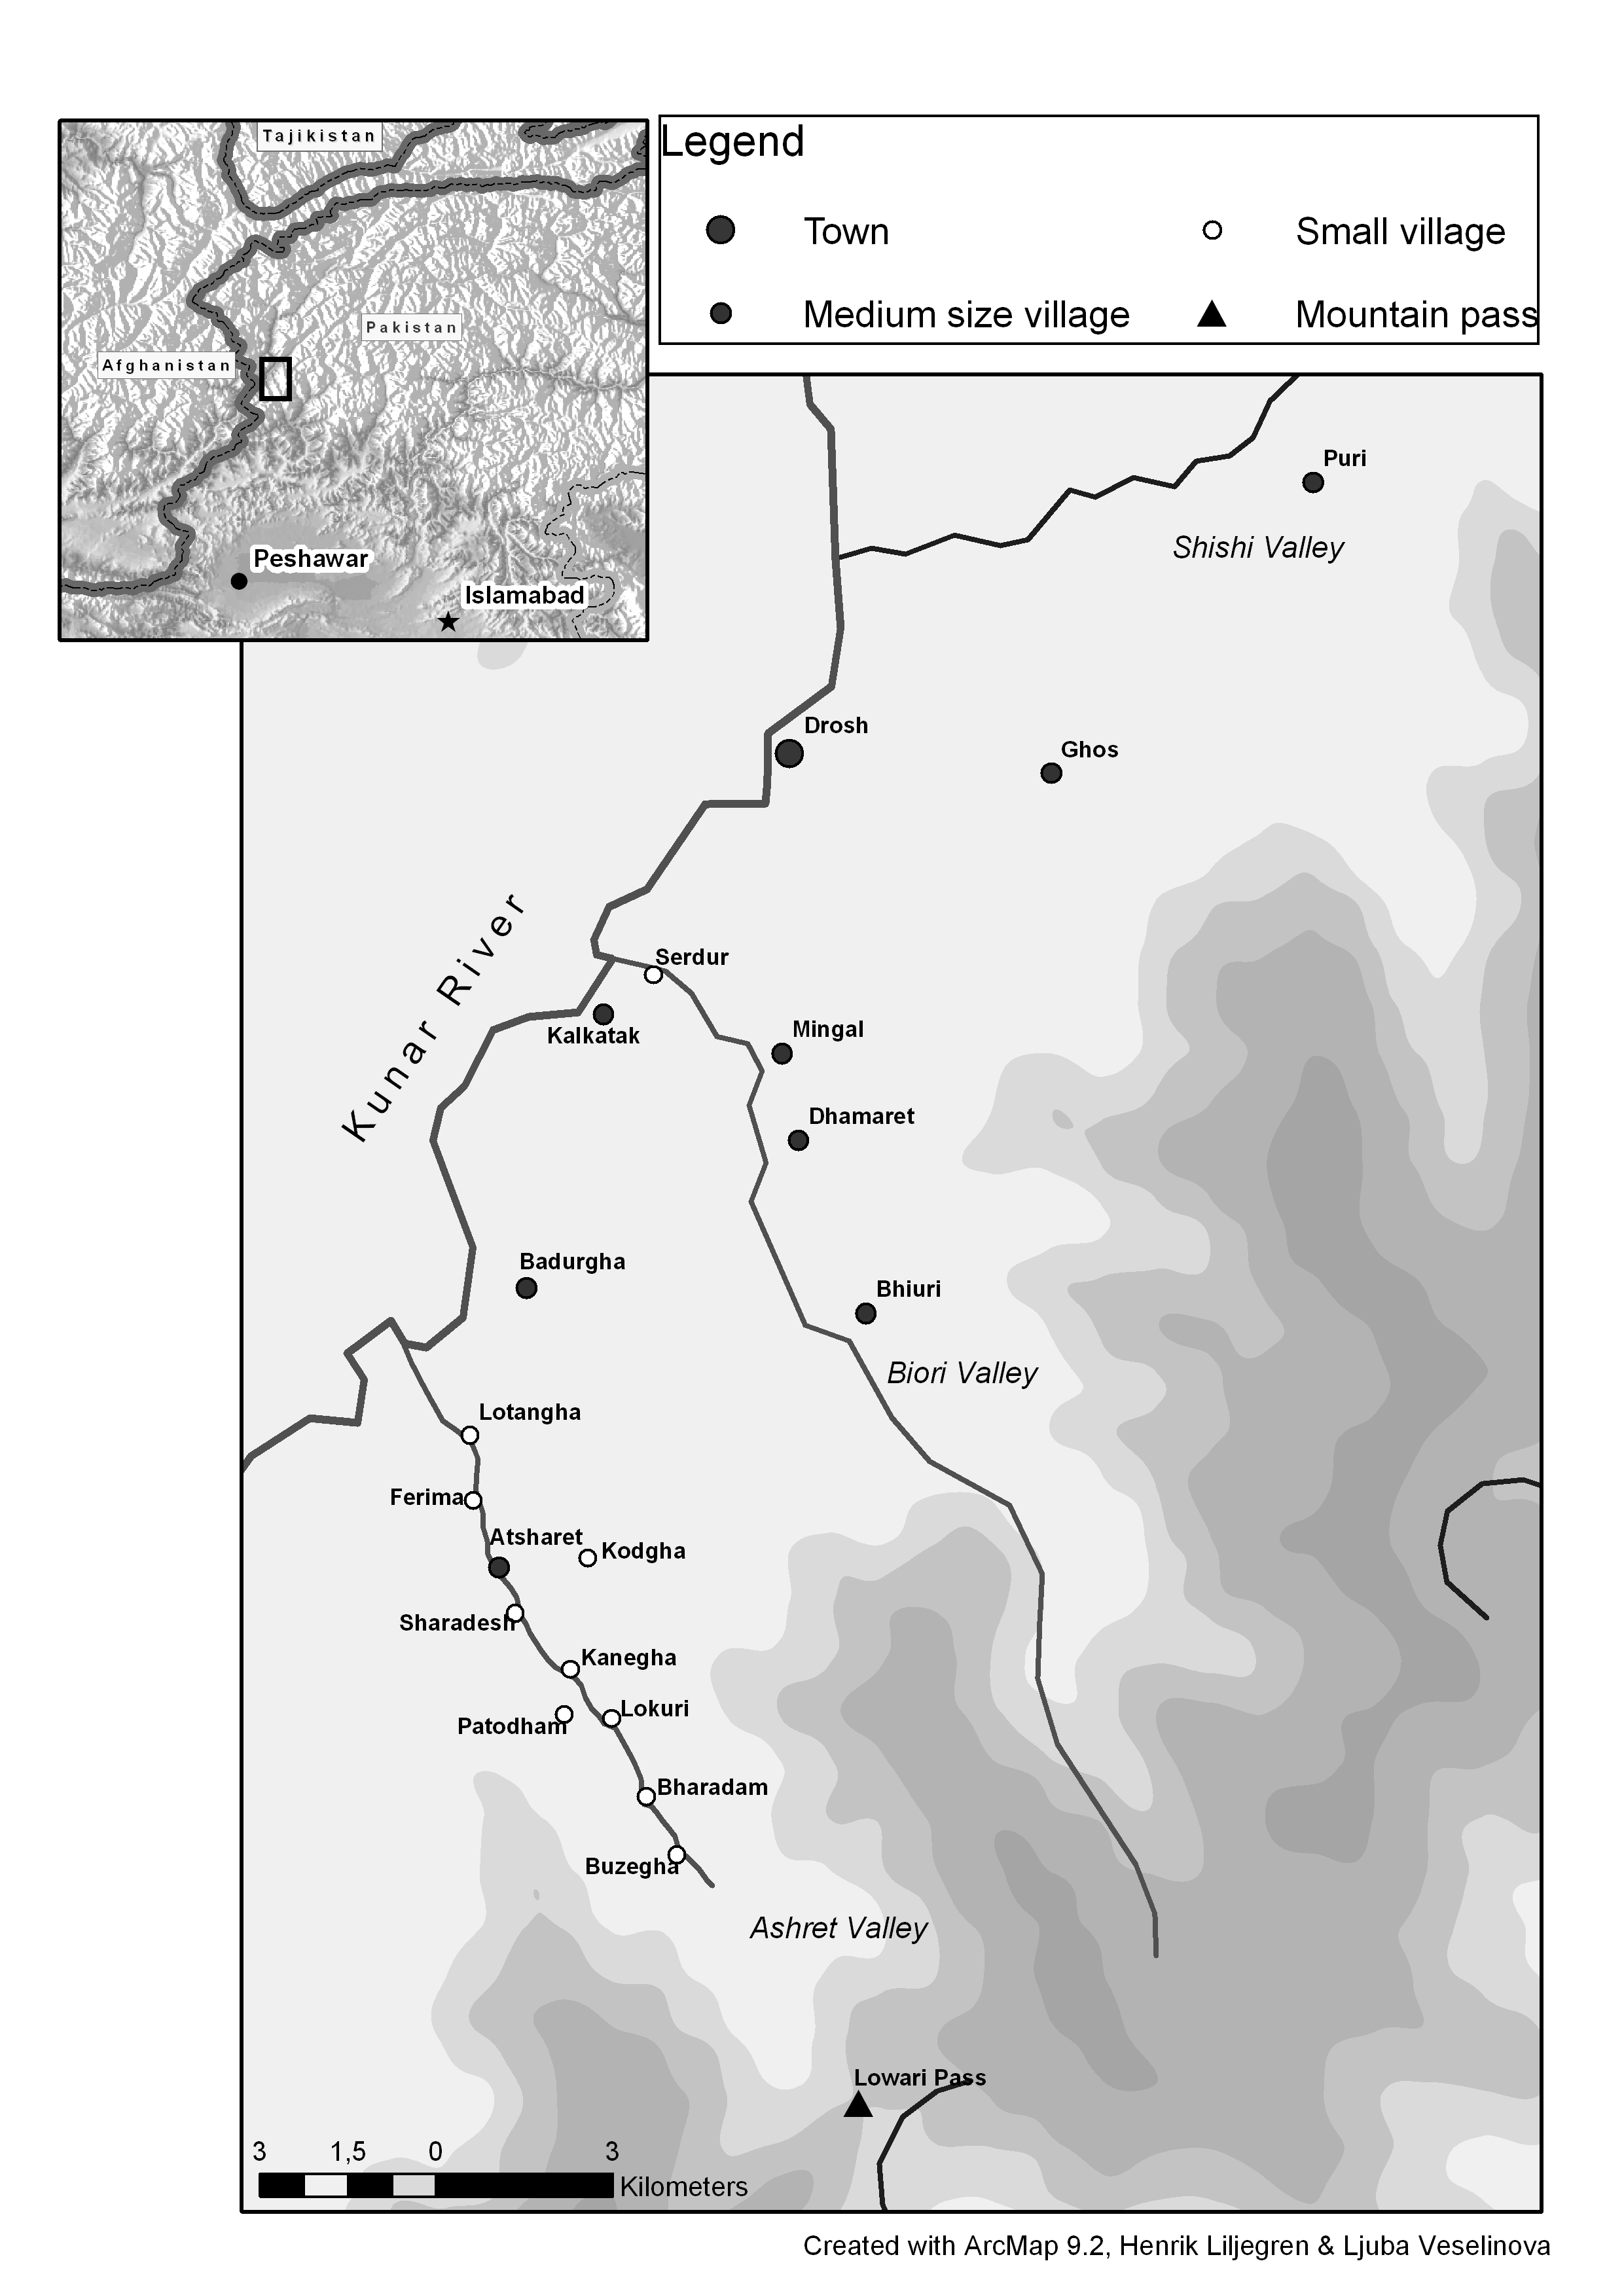
\includegraphics[width=.95\textwidth]{figures/ch1map1.png}
% \edcomm[inline]{Map 1 ist zu lang. Da müsste unten etwas von dem Weißen abgeschnitten werden.}
\label{map:1-1}
\end{mapfigure}


Four kilometres south of the bazaar town Drosh, the Biori Valley meets the main valley along the Kunar river. There are three distinct villages in this narrow side valley, which together with the Ashret Valley is to be considered the heartland of the Palula speaking community, all of them solidly Palula speaking: Mingál (or Lower Biori), Dhamareét (or Middle Biori), and Bhiúuṛi (or Upper Biori/Biori proper), the latter being the largest of the three, situated at an altitude of 1,800 metres. 


Apart from those two main settlements, there are a~few other non"=adjacent villages where Palula is also spoken, or at least has been spoken in the recent past. The northernmost of these villages is Purigal (Púri in Palula), which is situated about twenty kilometres north of Drosh, about seven kilometres into the Shishi Koh Valley. Once an~exclusively Palula"=speaking village, the language is now competing, more than likely on the losing side, with Khowar. The next location with a~substantial number of Palula speakers~-- though the number is markedly in decline~-- is Kalkatak (Galaṭáak), a~village situated in the fertile main valley, six kilometres by the main road south of Drosh, near the mouth of the Biori Valley. In this village, Palula competes primarily with Khowar, and to a~considerably lesser extent with Pashto, and the usage of Palula is dramatically decreasing in the younger generation. This may in some ways be the repetition of the scenario in this village about a~century ago, when Palula obviously won ground over the then dwindling Kalasha language (\citealt[165]{decker1996}; \citealt[95]{cacopardo2001}). The small village Serdur (Sawdár), situated right at the mouth of Biori Valley, where the majority is reported to speak Palula, is for official purposes treated as a~part of Kalkatak, but it is on the local level mostly considered a~separate unit (Fakhruddin Akhunzada, pc). On the arid mountainside a~couple of kilometres east of Drosh is a~small and remote village called Ghos (Ghoós), which apparently was Palula"=speaking in the recent past (\citealt[75, 84]{decker1992a}), but, according to an~informal survey carried out in 2005 by my local language consultants, it has switched entirely to Khowar. Another village that deserves to be mentioned is Badrugal (Baaḍurghaá), which is located in the main valley between Ashret and Kalkatak, and according to local sources is inhabited by a~substantial number of people able to communicate in Palula. The first language of most (male) villagers is given as Shekhani or Shekhwar, a~Nuristani language, but many have reportedly acquired Palula in frequent contact (especially through intermarriage) with the nearby Palula settlements. 


\begin{photofigure}[t]
\caption{Cluster of houses in Mingal, Biori Valley, 2002 (Dietmar Polster)}
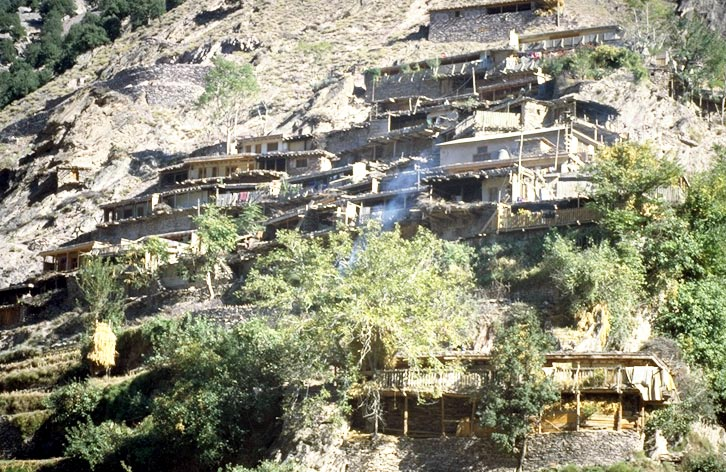
\includegraphics[width=\textwidth]{figures/ch1photo2.jpg}
\end{photofigure}


Outside of what is in a~strict sense part of the Palula"=speaking area in Chitral, one other place
that should be mentioned is a~village called Gumandand (Gumaaṇḍáṇḍ) in Dir Kohistan (in the
neighbouring Upper Dir District to the east). Previously, \citet[9]{morgenstierne1941} mentioned the
tribal connection between this village and the Palula of Chitral, and a~number of people in Ashret
have similarly pointed out that they indeed have relatives there, as a~result of a~past migration
from Ashret. However, I have yet to come across any solid evidence for the same or a~similar
language being spoken there. It is also unclear whether there is a~linguistic or tribal connection
between this village and another village in Dir Kohistan, namely Kalkot, where a~closely"=related
speech variety has been recorded (see \sectref{subsec:1-3-1} for a~discussion on the
relationship between the Palula of Chitral and the speech of Kalkot).


\begin{table}
\caption{Estimated number of Palula speakers in each location}
\begin{tabularx}{\textwidth}{ l l Q }
\lsptoprule
Location &
Speakers &
Comment\\\midrule
Ashret Valley &
5,899 &
Pashto"=speaking Buzeeghaa subtracted from a~total of 6,071 (2004)\\
Biori Valley &
3,000 &
Approximation based on number of households (2004)\\
Purigal &
\phantom{9}200 &
An estimated 50 per cent of the six to seven people in each of the 60 households (2004)\\
Kalkatak &
\phantom{9}541 &
Speakers counted (1998), includes Serdur\\
Badrugal &
\phantom{9}200 &
Rough estimate\\
\textbf{Total} &
\textbf{9,841} &
\\\lspbottomrule
\end{tabularx}
\label{tab:1-1}
\end{table}


As far as the total number of Palula speakers is concerned, we can only provide a~rough estimate at
best (shown in \tabref{tab:1-1}), due partly to the lack of any reliable census directly mapped
to language use, and partly to the changeable and multilingual situation of the region. Based on
a~combination of population data provided by a~local health network in Ashret, the results of
surveys carried out by the local ethnographer and sociologist Fakhruddin Akhunzada in Biori and Kalkatak,
interviews with local respondents in Purigal, and an~assumption that there are a~couple hundred
speakers of Palula in Badrugal (out of a~total population of 740 in 1987 according to
\citealt[143]{decker1992a}), we conclude that there are approximately 10,000 speakers of the
language in Chitral, a~figure that should be treated with a~certain amount of healthy
scepticism.\footnote{The seemingly exact figure 8,600 that \citep[74--76]{decker1992a} arrived at
  (later cited by Ethnologue) was in fact also the result of quite a~rough estimate, based on
  a~combination of respondent opinion and a 1987 census report.} Provided there has been no dramatic increase in any of the other speech communities in the district, Palula is still the second largest language community in Chitral, as it was according to a~survey carried out in the 1990s (\citealt[11]{decker1992a}). 

\subsection{The socioeconomic environment}
\label{subsec:1-2-2}

All of the locations with any higher concentration of Palula speakers are villages with a~rudimentary infrastructure. The community is mainly agricultural, often combined with animal husbandry, and its inhabitants also receive income from timber harvesting, in the form of royalties on the cedar forest and through the sale of firewood. The main subsistence crops cultivated are wheat and maize, but also a~variety of fruit and vegetables is grown. In most of the villages there is an~ample supply of water for irrigation. A portion of the population in the Ashret Valley, as well as in the Biori Valley, practice transhumance, in the spring taking their herds of sheep and goats to the high pastures situated at the extreme ends of these valleys and staying there throughout the summer months. This practice, and interrelated activities such as the production of a~large variety of dairy products, was a~central part of community life and traditions but has given way to today's mainly agricultural society. Whereas irrigated land in and adjacent to the villages and nearby winter pastures are owned by individual families, the distant summer pastures are communal.


As the educational level is steadily increasing and the demand for an~income source besides agriculture is deemed necessary, a~growing number of people are being employed by the government or carry out business within the private sector, either in their home village, e.g., as school teachers, or in the bazaar town Drosh or in Chitral town, the administrative centre of the district. There is also a~local bazaar in Ashret proper, occupying a~smaller number of shopkeepers and craftsmen from the valley. In pursuit of other employment opportunities, a~number of Palula families have migrated to urban areas, settling more or less permanently in larger cities such as Peshawar, Rawalpindi and Lahore.
 
\subsection{Local history and cultural identity}\label{Local history and cultural identity}
\label{subsec:1-2-3}
% \authcomm{If possible I would like to include another photo. It was originally used as the front cover of my PhD dissertation and is taken during a wedding ceremony in Ashret in June 2005.}
% \edcomm{inserted dummy for that photo}
\begin{photofigure}
 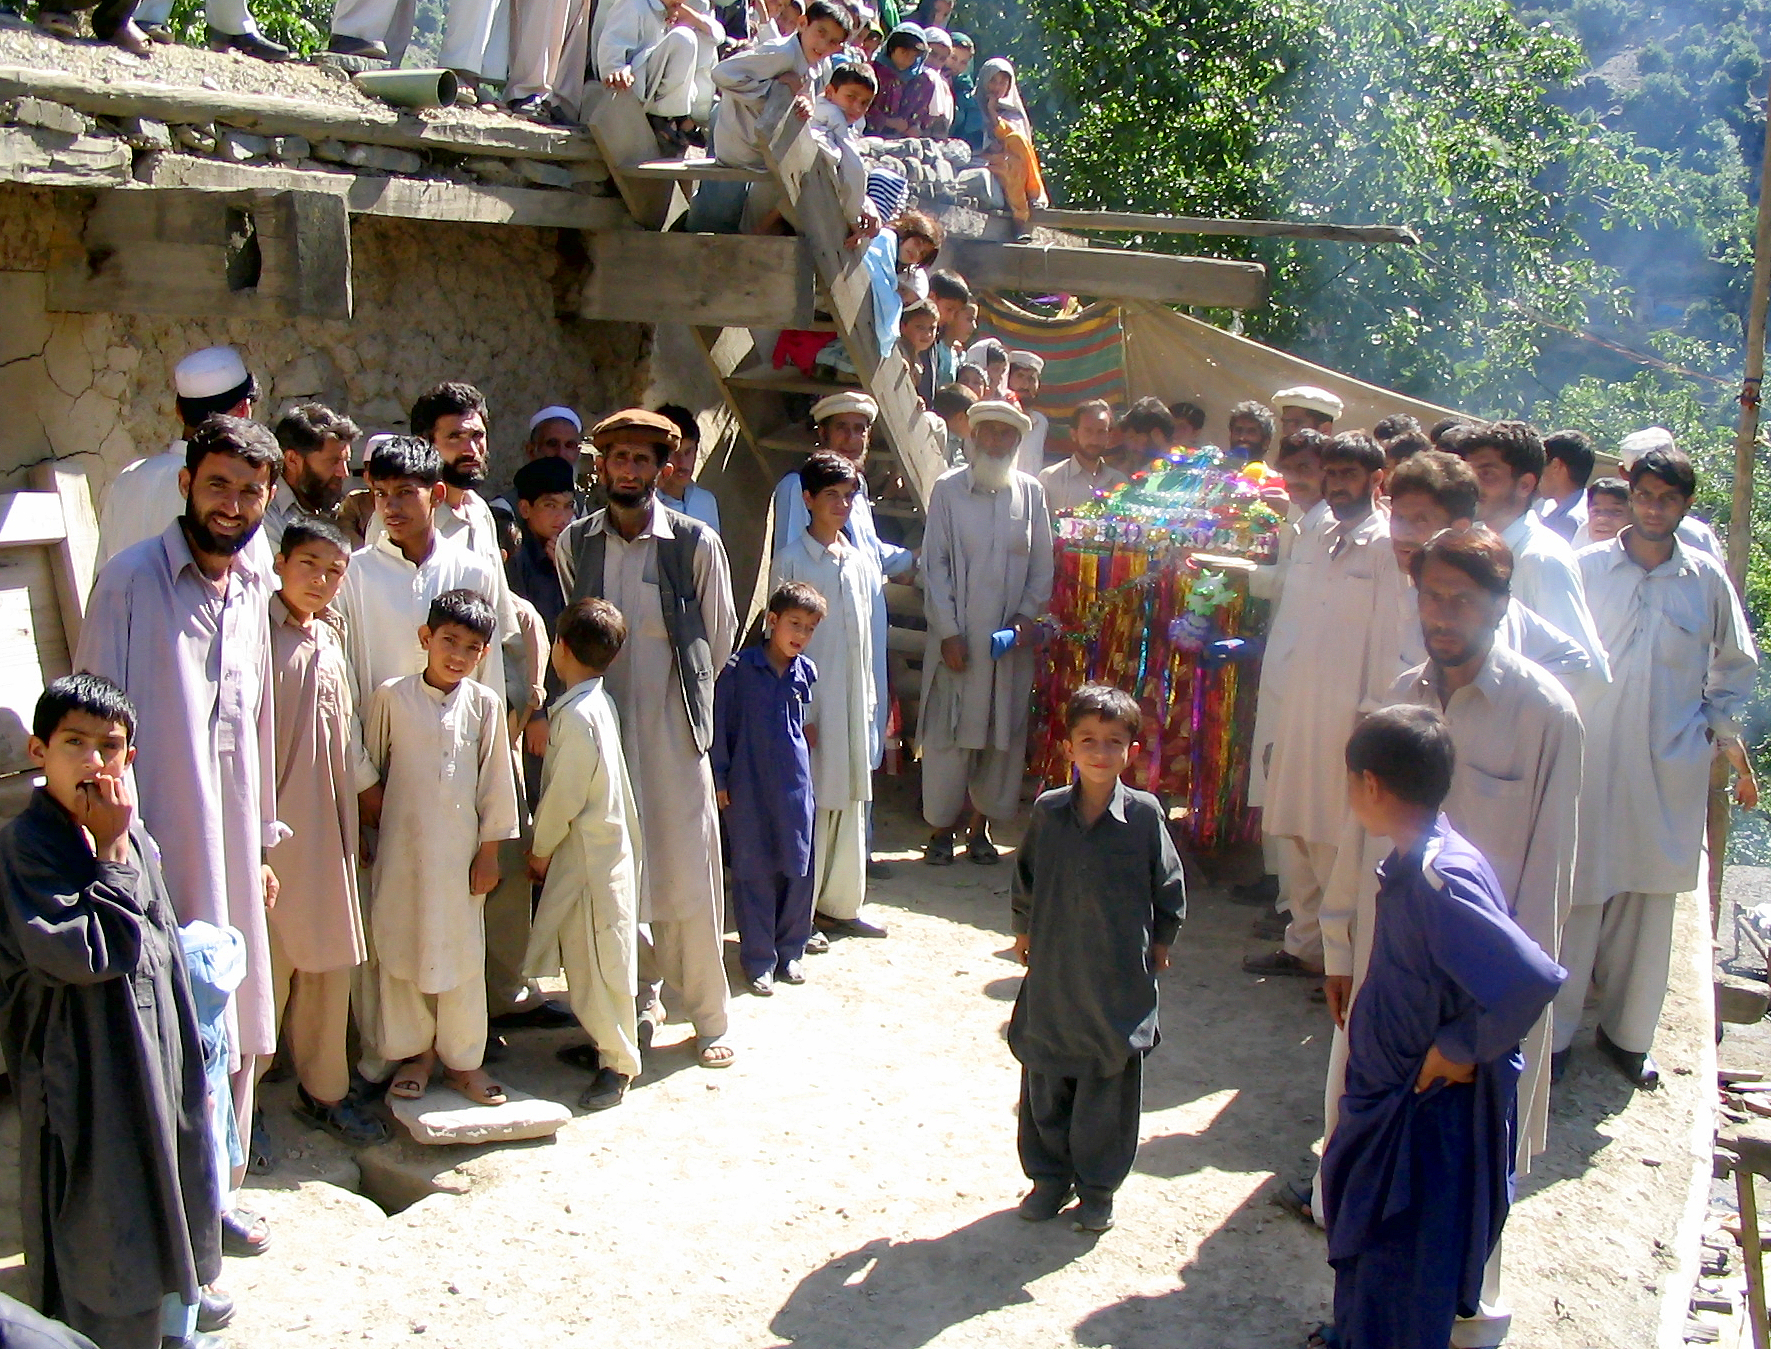
\includegraphics[height=.3\textheight]{photos/Photo02--WeddingAshret.JPG}
\caption{Wedding ceremony in Ashret, 2005 (Henrik Liljegren)}
\label{fig:1:weddingphoto}
\end{photofigure}


Palula has usually been described or seen as a~single"=language community (\citealt[7]{morgenstierne1941}; \citealt[67]{decker1992a}; \citeyear[160]{decker1996}; \citealt[21]{masica1991}; \citealt[253, 258]{strand2001}) as well as a~single"=ethnic community (\citealt[79--143]{cacopardo2001}; \citealt[5]{akhunzadaliljegren2009}). Although the former is not very surprising, considering the relatively minor dialectal differences, the latter is a~more complex issue. From the outsider perspective, and more specifically from the perspective of the Khowar speaking majority of Chitral District, the people and the speech of the Ashret and Biori Valleys are indistinguishable, and they refer to the people as a~whole as the Dangarik and their speech~-- dramatically different from their own language~-- as Dangarikwar. Internally, however, the picture is less clear. Indeed, from the perspective of the ``southerners'' in Ashret, the speech of the ``northerners'' in Biori is rather similar and largely comprehensible, and vice versa, but from both sides the idea is also common that the other variety is a~speech form that is somehow debased or has deteriorated from its pure or original form. Although speakers of the two varieties have interacted and to some extent have also intermarried for a~long time, it is obvious that the community in Ashret do not consider the community in Biori to be related to them, the main reason being that they have no genealogy in common. 


As is the case in many other communities in the region, there are preserved oral traditions concerning a~particular place of origin in these communities as well as genealogies memorised from generation to generation. The most extensive and consistent traditions of this kind is found in Ashret,\footnote{These traditions, including the important historical manuscript Tarikh-i-Ashret, written by the local poet and historian Mirza Guldali Shah in Persian verse, are commented on at great length and in great detail by \citet[79--143]{cacopardo2001}, and a~translation of it into English is included in its entirety as an~appendix to their work.} where the entire population claims descent from a~common ancestor. 


According to local history, the ancestor of the people of Ashret was Choke (C̣hoók), son of
Machoke (Mac̣hoók),\footnote{In some versions of this tradition, Choke and Machoke were brothers
  (\citealt[85]{cacopardo2001}, and my own notes).} who migrated to the present location from
Chilas in the Indus Valley some fifteen to sixteen generations ago, a~scenario convincingly corroborated by
recent research into local history and culture carried out by the anthropologist Alberto Cacopardo
\citep[84--93]{cacopardo2001}. One particular source states how Choke and two of his brothers
arrived in Chitral and reached Drosh but subsequently separated. One brother went to Kalas,
a~village in the Shishi Koh Valley north of Drosh, another continued to Sau in the Kunar Valley (in
present"=day Afghanistan), where he settled, and Choke himself settled in Ashret
\citep[84]{cacopardo2001}. This would support a~common origin of the Palula speakers of Ashret and
the inhabitants of Sau, the language of the latter closely related to Palula.\footnote{This was
  confirmed by respondents from Sau interviewed in an~Afghan refugee camp in Dir in 2000 by Ajmal
  Nuristani and myself who stated that ``the people of Ashret are our brothers''.} The inhabitants
of present"=day Kalas, on the other hand, are all Khowar speakers, but according to respondents in
Puri (the only remaining Palula"=speaking village in Shishi Koh Valley), the people of Kalas formerly
spoke Palula. An independent local tradition among the Bozhokey in the Laspur Valley (about 200 km
northeast of the Palula"=speaking area) also speaks of a~migration from Chilas some twelve to fifteen
generations ago. Inayatullah Faizi, himself a~Bozhokey, has documented this tradition, according
to which the two brothers Choke and Machoke left Chilas after a~power struggle with their elder
brother, and after having parted during their exile, Machoke arrived in Laspur where his elder son,
Laphur, subsequently settled. The descendants in the Laspur Valley have since been linguistically
assimilated by their Khowar"=speaking neighbours. Also, some Ashreti sources claim that the Chilasi
immigrants indeed came to Ashret from the north, perhaps via Laspur, rather than through the Lowari
Pass and Dir Kohistan, which would agree with this Laspuri tradition \citep[85, 125--126]{cacopardo2001}.


What then about the Palula speakers in Biori? They are not mentioned in any of the migration
traditions from Ashret (or those agreeing with it), whereas it has been explicitly pointed out to me
by Ashretis that the people of Biori are descendants neither of Choke nor Machoke but are Kohistanis
from Dir who later adopted the language of Ashret (compare \citealt[255]{strand2001};
\citealt[296]{saeed2001}). The first part of the statement can very well be true, as the main Biori
genealogies lack any convincing links to the genealogies of Ashret, but I suspect the second part to
be an~overinterpretation on the part of the Ashreti informants. Although the ethnic composition of
the Biori Valley population is much more complex (including considerable sections with Kalasha and
Nuristani origin), and with much less consensus around its origin than what is the case in Ashret,
there is indeed a~local tradition that connects a~major section of the population (especially in the
uppermost village Bhiúuṛi) with Dir Kohistan, in particular with a~village called Biyar
(Bhiáaṛ). Although somewhat speculative, it is possible that a~genitive or perhaps an~adjectival
form along with a~regular sound change from ‌/aː/ to /uː/ would render the form Bhiúuṛi,
i.e., `from Biyar'. Also \citet[111--108]{cacopardo2001} draws the conclusion that the
Palula\footnote{Keeping in mind that the ancestors of a~good portion of the ethnically"=mixed
  population most likely were speakers of a~variety of Kalasha, and that there may also have been
  other linguistic enclaves before Palula became the sole surviving language of the valley.} of
Biori most likely came to the valley from Dir Kohistan, somewhat later than the Palula of Ashret,
possibly to escape conversion to Islam, which was common at the time in Dir Kohistan. While
present"=day Biyar is a~Kohistani (Gawri"=speaking) village, and there are no obvious traces of any
previous language spoken in the village, it is not wholly unlikely that the population speaking
a~language closely related to Palula in the relatively close village Kalkot (both being situated
along the Panjkora river) is a~remnant of a~once more widely spoken Shina variety in this part of
Dir Kohistan. Muhammad Atiqullah, a~local historian and also my main language consultant in Biori, further
claims that the people who came from Biyar were originally from Tangir, one of the Indus side
valleys west of Chilas (hence the name Tangiri/Dangarik as mentioned
earlier).\footnote{Interestingly, while Ashreti people usually dislike the Chitrali designation
  Dangarik or Dangarikwar, the people of Biori do not seem to mind and sometimes even use the term
  referring to their own community.} In Puri (also part of the same general dialect area as Biori),
a~local elder told me that their village was founded by two brothers, Dúuši‌ and ‌Kaṇúuši, who came
via Dogdarra, a~valley in Dir Kohistan, from a~village in the Tangir Valley called Dangeri Phuruṛi,
possibly corresponding to a~very real place in central Tangir that is rendered Phurori on some
maps. As a~possible explanation for the exclusiveness on the part of the Ashretis vis-à-vis the
Palula speakers of Biori, Inayatullah Faizi (pc) has suggested that those ancestors of the Biori
Palula who came from Dir Kohistan may very well have been Shina speakers, but being Yeshkun rather
than Shin\footnote{According to \citet[17]{jettmar2002}, the population in the traditional Shina
  territory was organised into four castes~-- Shins, Yeshkuns, Kamins and Doms~-- with the Shins
  considering themselves ritually cleaner than the other three, possibly modelled on Hindu
  communities in adjacent areas. } would immediately have placed them in a~non"=kin category,
regardless of the their linguistic relatedness.\footnote{This idea, however, is disputed by Alberto
  Cacopardo (pc), who holds that the awareness of such a~caste identity in relatively recent times
  is out of question.}


What this gives us are (at least) two possible migration routes from the Indus Valley to
Chitral. One would have originated in the Chilas area, in the main Indus Valley, taking the way over
the Shandur Pass to Laspur and then continuing south through Chitral to the Ashret Valley, branching
out quite early on to Sau in the Kunar Valley. The other one would have originated in the Tangir
Valley,\footnote{As rightly pointed out by Alberto Cacopardo (pc), there is a~narrow, modern"=day use
  of Tangir that refers to a~particular side valley to the west of Chilas in the Indus Valley, but
  there is also a~broader, past use of Tangir that refers to the larger region around Chilas,
  including many of the major areas where varieties of Shina are spoken.} taking the route over
Swat and Dir Kohistan, leaving a~trace in Kalkoti speech, and ending up in the Biori Valley. Whether or
not there is any linguistic evidence supporting this hypothesis is something we will have reason to
return to briefly below (\sectref{subsec:1-3-1}).


The arrival of the Palula in Ashret must, if the local genealogical evidence and other historical
traditions are taken into account, be dated to some time before the mid-17th century \citep[88]{cacopardo2001}, and the migration from Dir Kohistan to Biori somewhat later
(\citeyear[118]{cacopardo2001}). As for the religion of the Palula speakers, they were clearly still
unconverted to Islam when they first entered Chitral, and it was probably not until the latter half
of the 19th century that they embraced Islam (\citeyear[83]{cacopardo2001}), and
even then only gradually and probably earlier in Ashret than in Biori. What kind of religion was
practiced before the Muslim conversion remains uncertain, but elements in it are shared with the
non"=Muslim Kalasha as well as what is known about other pre"=Islamic religions in the region. Finally, I will quote Alberto Cacopardo's brief but interesting summary of his own findings about the great"=grandfathers of today's Palula:

\begin{quote}
They were goat"=herders, whose women in the summer watered the fields, while the men went up on their
own to the high pastures. Cows were impure to them, like the women at the time of seclusion. They
had something like a~priestly lineage, and some of them held feasts of merit. They lived in densely
forested valleys haunted by murderous bandits and by the fear of monstrous ghosts. They were mostly
dressed in goatskins and travelled only on foot, but they remembered ancestors who rode on horses
and fought with bows and arrows against princes who lived in forts. They had rites in which they
drank wine and men and women danced together at night. They had temples and shrines, sacred stones
and wooden idols, and they said they heard the voices of the fairies \citep[143]{cacopardo2001}.
\end{quote}

\section{The linguistic setting}
\label{sec:1-3}
\subsection{Genealogical affiliation}
\label{subsec:1-3-1}
Palula belongs to a~group of Indo"=Aryan (IA) languages spoken in the Hindukush region that are often referred to as ``Dardic'' languages. Totally 27 named varieties are sorted under this grouping \citep{ethnologue2015}. It has been and is still disputed to what extent this primarily geographically defined grouping has any real classificatory validity.\footnote{For an~overview of the terms Dard, Dardic and Dardistan and their different uses, see \citealt{mock1997}.} On the one hand, \citet[251]{strand2001} suggests that the term should be discarded altogether, holding that there is no justification whatsoever for any such grouping (in addition to the term itself having a~problematic history of use), and prefers to make a~finer classification of these languages into smaller genealogical groups directly under the IA heading, a~classification we shall return to shortly. 

\begin{sidewaysfigure}[p]
\caption{Languages in the Hindukush region}
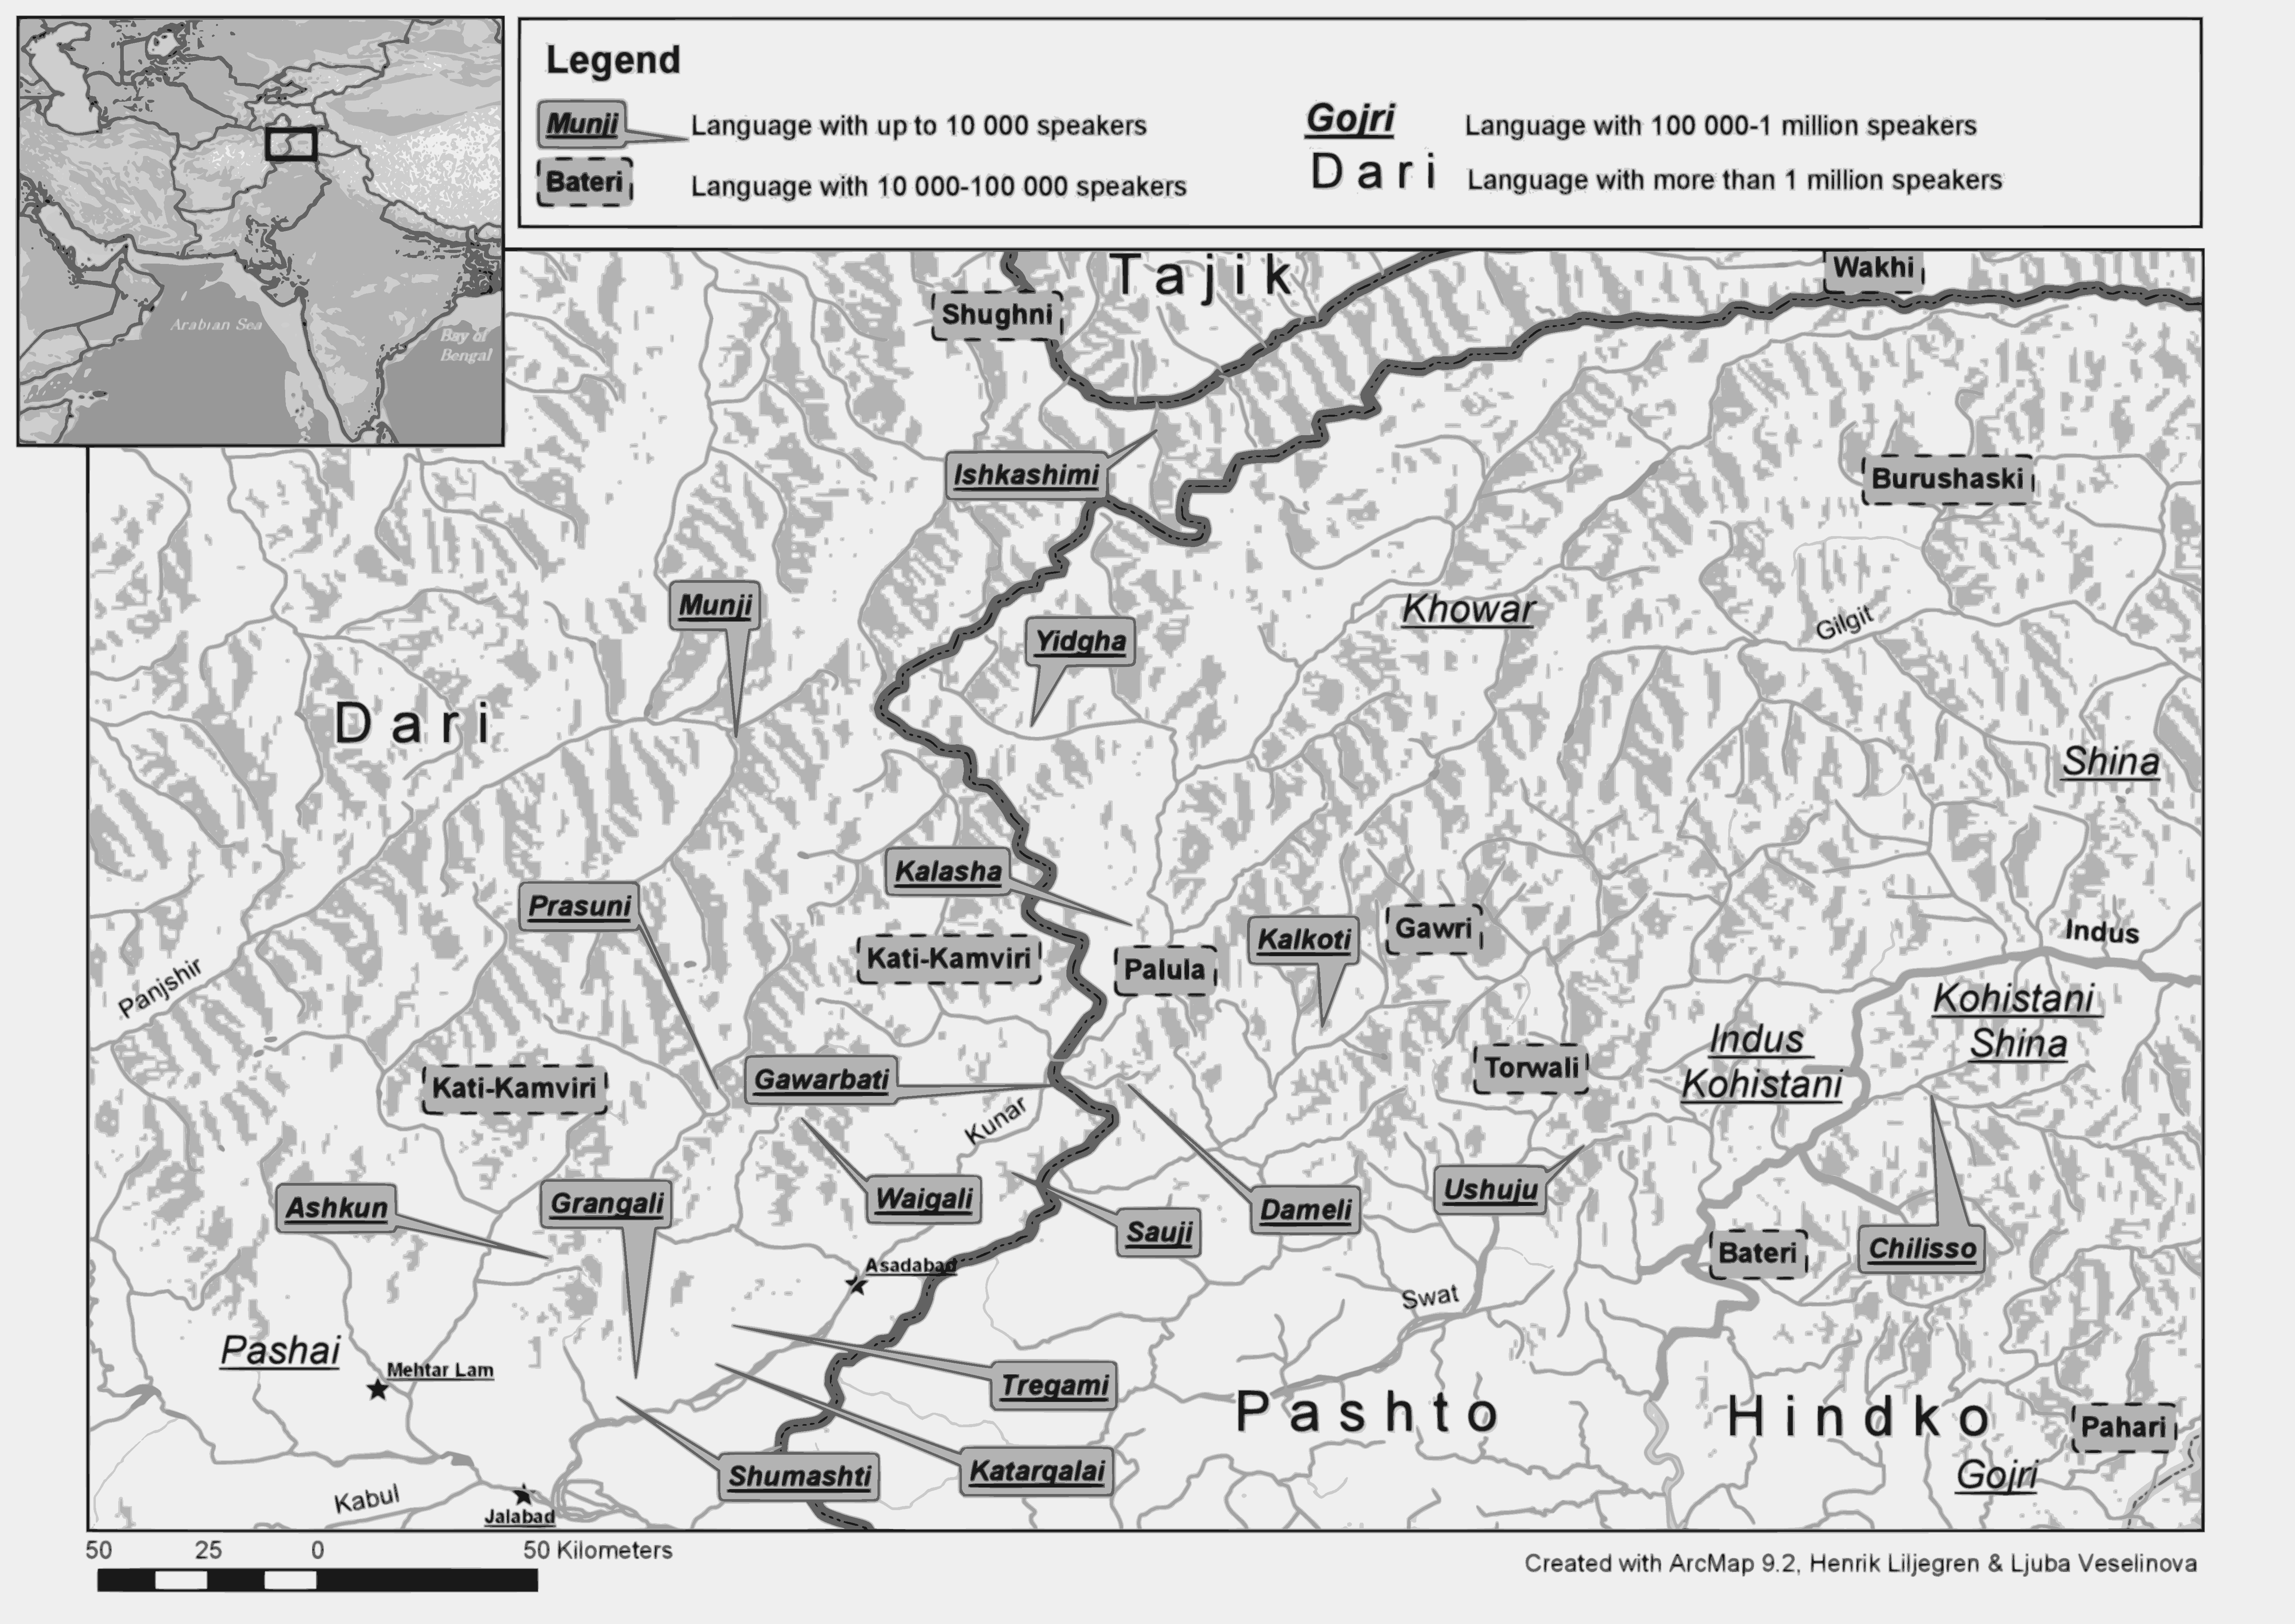
\includegraphics[width=.8\textwidth]{figures/ch1map2.pdf}
\label{map:1-2}
\end{sidewaysfigure}

% \authcomm{The map (1.2) seems to be misaligned, too far into the left margin}
Others have continued using the term, for various reasons, in a~classificatory sense. \citet[822]{bashir2003} concludes that there are enough similarities across these languges, in terms of shared retentions, areal features and innovations affecting at least subsets of the languages to justify the umbrella term ``Dardic'' even though she expresses doubt about the possibility of tracing them all to a~single node in a~Stammbaum model. \citet[10--11]{zoller2005} identifies the Dardic languages as the modern successors of the Middle Indo"=Aryan (MIA) language Gandhari (also Gandhari Prakrit), but along with Bashir, Zoller concludes that the family tree model alone will not explain all the historical developments. 


\citet[460]{masica1991} questions the value of trying to sort out a~complete and accurate New Indo"=Aryan (NIA) historical taxonomy and contends that it would be far more interesting to focus on and recognise a~number of overlapping genealogical zones, some of them more strongly defined than others. Following that position, I will in the remainder of this work refer to these languages as Hindukush Indo"=Aryan languages (HKIA), without any claim of taxonomical correctness but recognising the shared historical developments pointed out by Bashir and Zoller. 


Some words should now be said about the lower"=level grouping of these HKIA languages, which have as their home an~extremely mountainous region that stretches from north"=eastern Afghanistan over northern Pakistan all the way to Kashmir (see Map~\ref{map:1-2}). \citeauthor{strand2001} recognises in his classification (\citeyear[258]{strand2001}, which represents an~updated and corrected version of \citealt{strand1973}, which in its turn is based on the work of Morgenstierne) eight groups (some of them represented by one language alone): 

\begin{enumerate}
\item \textit{Pashai}, with a~western and an~eastern dialect cluster, is spoken in an~area north of Kabul River in Afghanistan, close to the Pakistani border. The Ethnologue (\citeyear{ethnologue2015}) and Glottolog (\citeyear{glottolog2015}) identification of four distinct Pashai languages is based on Morgenstierne's (\citeyear{morgenstierne_pashai1973}) division of Pashai into South-Western [psh], North-Western [glh], South-Eastern [psi] and North-Eastern Pashai [aee].


\item \textit{Pech group} includes the languages Gawarbati [gwt], Grangali [nli] and Shumashti [sts], of which the latter two are seriously threatened. Grangali and Shumashti are spoken in the same general area as Pashai, and Gawarbati is spoken in the Kunar Valley on both sides of the Afghan"=Pakistan border. 


\item \textit{Pech"=Kunar group}, which as a~group is merely hypothetical, consists of one known language, Katarqalai [wsv] \citep{buddruss1960}, perhaps still spoken in one single village in the lower Tregam Valley, not far from the main Kunar Valley in Afghanistan. \citet[825]{bashir2003} places it in the Kohistani group.


\item \textit{Chitral group}, with its two languages Khowar [khw] and Kalasha [kls], which are both spoken in Chitral District in Pakistan.


\item \textit{Tirahi} [tra], which is perhaps no longer spoken, is the language of a~few villages southeast of Jalalabad in Afghanistan \citep{morgenstierne_tirahi1934}. \citet[824]{bashir2003} places this language in the Kohistani group.


\item \textit{Kohistani group}, includes a~number of rather diverse languages at the centre of the HKIA region. \citet[258]{strand2001} places Dir/Kalam Kohistani (or Gawri) [gwc] and Dameli\footnote{An entirely accurate classification is still lacking. \citet[824]{bashir2003}, for instance, groups Dameli with Gawarbati in a~Kunar group.} [dml] in a~western cluster, the former spoken in Dir and Swat Kohistan and the latter in southern Chitral. In an~eastern cluster we find Indus Kohistani [mvy], Gowro [gwf], Chilisso [clh] and Bateri [btv], all spoken in the Indus Valley, and Torwali [trw] in upper Swat.


\item \textit{Kashmiri} [kas], with its two main dialects Kashtawari and Poguli, is spoken in Kashmir. 


\item \textit{Shina}, where the closest relatives to Palula are found, is traditionally described as one language with different dialects, but in actual fact it covers a~number of rather diverse and geographically widespread varieties \citep[17]{schmidt1985}, spoken by a~range of ethnic groups, from the Kunar Valley in Afghanistan all the way to Kashmir (with its largest uninterrupted area along the portion of the Indus stretching from Kohistan district in the south, through Chilas District, covering the east"=west flowing portion of the river, then in Gilgit"=Baltistan branching out both eastwards into the Skardu area of Baltistan and westward along the Gilgit River). Strand identifies two main clusters, a~Chilasi cluster and a~Gilgiti one:

\begin{tabbing}
Chil\=Kohistanddi\=\kill
Chilasi \\
\>Kohistani Shina [plk] \\
\>Eastern dialects \\
\>\>Astori \\
\>\>Drasi \\
\>Dispersed dialects \\
\>\>Palula [phl] \\
\>\>Ushojo [ush] (?) \\
\>\>Kalkoti [xka] (?) \\
Gilgiti [scl] \\
\>Brokskat [bkk] (a Tibetanised offshoot) \\
\end{tabbing}
\end{enumerate}

In an ambitious survey of Shina dialects, Radloff (\citeyear{radloff1992}) obtained and compared word lists from 27 different locations (including only what she, implicitly, regarded as representatives of Shina proper, and thereby excluding obvious ``outliers'', such as Palula at the Western extreme and Brokskat at the Eastern extreme), and came to the conclusion that Shina, on the one hand, can be divided into four clusters based on geographical proximity (Northern, Eastern, Diamer and Kohistan), and on the other hand, can be sampled into two major centres, one around Gilgit and the other around Chilas. A continuum, with two end points, Gupis and Kolai, as described by Radloff (\citeyear[132]{radloff1992}), corresponds quite well to the full extension of Shina-speaking locations along the Gilgit/Indus river system, an analysis which in many ways also justifies the labels [scl] and [plk] chosen to pinpoint two markedly different poles with a great number of intermediate forms, particularly realised in the varieties that Strand labels ``Eastern dialects''.      


Strand further identifies the dispersed and archaic varieties Palula and Sawi [sdg] (or Sauji) as of particular interest (the reason he does not include Sawi in the list is perhaps that he sees Palula and Sawi as basically one and the same variety), and that two other speech enclaves, Ushojo and Kalkoti, probably should be included as well (his question marks indicating the need for more and better data in order to draw reliable conclusions). Yet another distinct variety that would be a highly likely candidate for inclusion under ``dispersed dialects'' is the language of Kundal Shahi [shd], a speech variety of a small community residing in the Neelum Valley in Pakistan-administered Kashmir \citep{baartrehman2005}.


It is primarily in a~phonological comparison between cognates that Palula appears to be conservative vis-à-vis the other Shina varieties (\tabref{tab:1-2}). In a~comparative study between some major varieties (Palula not included), \citet[36]{schmidt2004} shows that three features are common to all of them: a) the preservation of the OIA three sibilants \textit{s, š, ṣ}, as in HKIA languages in general, b) the development of retracted (retroflex) fricatives \textit{c̣} and \textit{ẓ} from OIA clusters \textit{tr, kṣ, dr, bhr,} etc., and c) the development of contrastive pitch accent. While Palula shares the first and the third of those with the other varieties, it has to a~larger extent preserved consonant clusters. 


\begin{table}[ht]
\caption{Comparison of cognates in five Shina varieties (based on \citealt[37]{schmidt2004}, with Palula (A variety) data added)}
\begin{tabularx}{\textwidth}{ l l X l X l l }
\lsptoprule
OIA &
Gilgiti &
Kohi\-stani &
Drasi &
Brok\-skat &
Palula &
\\\midrule
\textit{ɡōṣṭhá-} &
\textit{ɡoóṭ} &
\textit{ɡóoṣ} &
\textit{ɡoóṣ} &
\textit{ɡoóṣ} &
\textit{ɡhoóṣṭ} &
`house'\\
\textit{kr̥ṣṇá-} &
\textit{kíno} &
\textit{kíṇo} &
\textit{kíṇo} &
\textit{kyóno} &
\textit{kriṣíṇu} &
`black'\\
\textit{kárman-} &
\textit{kom} &
\textit{kom} &
\textit{krom} &
\textit{krum} &
\textit{kráam} &
`work'\\
\textit{kṣ\'{\={e}}tra-} &
\textit{c̣héec̣} &
-- &
\textit{c̣héec̣} &
-- &
\textit{c̣híitr} &
`field'\\
\textit{bhr\'{\={a}}tr̥-} &
\textit{ẓáa} &
\textit{ẓáa} &
\textit{ẓáa} &
-- &
\textit{bhroó} &
`brother'\\
\textit{*ǰāmātra-} &
\textit{ǰamac̣oó} &
\textit{ǰamc̣ó} &
\textit{ǰamac̣oó} &
\textit{ǰamó} &
\textit{ǰhamatroó} &
`son"=in"=law'\\
\textit{divasá} &
\textit{déez} &
\textit{dées} &
\textit{dées} &
\textit{dis} &
\textit{deés} &
`day'\\\lspbottomrule
\end{tabularx}
\label{tab:1-2}
\end{table}

\largerpage 
Something should be said about two of the other so"=called ``dispersed dialects'', Sawi/Sauji and Kalkoti, and their relationship to Palula. 


\textit{Sauji} (the form used by my respondents when referring to their language in contrast to
Sawi, which is the way it has been referred to in most literature) is the speech variety of Sau,
a~village situated in Afghanistan, on the east bank of the Kunar River, about 20 kilometers south of
the Pakistani border town Arandu in southern Chitral. It is uncertain to what degree and by how many
people Sauji is spoken today in this village, but according to \citeauthor{decker1992a}'s
(\citeyear{decker1992a}) informants, approximately 8,000--12,000 lived in the village prior to the
long period of war and unrest in Afghanistan.\footnote{A good portion of a~refugee camp in Timargira
  in district Dir that I visited along with Ajmal Nuristani in 2000 was made up of Sauji"=speakers
  from Sau. However, in the last few years many are said to have returned to their home village in
  Afghanistan.} That the variety spoken in Sau is closely related to Palula was pointed out
previously by Morgenstierne in the first half of the last century \citep[7]{morgenstierne1941}, and
was further confirmed by the more extensive study of the language undertaken by Buddruss in the
1950s:

\begin{quote}
Dagegen ist die nahe Verwandtschaft des Sawi mit dem Phal. bereits durch einen Blick in Grammatik und Vokabular evident und wird überdies durch die Angabe meines Gewährsmannes bestätigt, daß er die Sprache der Leute von Ashret verstehen könne. Dennoch sind die beiden Sprachen keineswegs identisch mit einander. (The close relationship of Sawi with Phal. is, however, already evident by a glance at its grammar and vocabulary, and is also confirmed by my informant's own statement, i.e., that he could understand the language of the people of Ashret. Yet, the two languages are by no means identical to each other. \textit{HL's translation.}) \citep[11]{buddruss1967}
\end{quote}


That there is a~historical connection between Sau and Ashret according to local tradition was
already mentioned (see \sectref{subsec:1-2-3}), but no major interaction or
contact between the two communities seems to have taken place in the recent past, and for a~long
time, the population of Sau has been included and been seen as a~part of the all"=surrounding Gawar
community, sharing their identity in all aspects save the language, something rather remarkable from
a~regional perspective \citep[232]{cacopardo2001}.
 
\textit{Kalkoti} (or Khalkoti), on the other hand, has remained largely undocumented. It is spoken by approximately 6,000 people, apparently confined to a~village called Kalkot, situated in the upper Panjkora Valley in Dir Kohistan. Since no systematic survey has been carried out in Dir Kohistan, however, it is too early to exclude the existence of other locations where this variety or something similar is spoken. Most other villages in the main valley, from Rajkot (Patrak) and upstream, are Gawri"=speaking,\footnote{I use Gawri to refer to the Kohistani varieties that have been variously called Bashkarik, Kalam (Kalami) Kohistani or Dir Kohistani. Gawri seems to be the preferred name and one that can be accepted by speakers from locations both in Swat and Dir Kohistan.} but that the speech of this village\footnote{In fact, 
  about 70 per cent of the Kalkot population are speakers of Kalkoti, whereas the remaining 30 per cent are speakers of a~Gawri variety (Muhammad Zaman Sagar, pc).} could be something rather different was first hinted at in a~sociolinguistic survey carried out by \citet[7]{rensch1992} and his colleagues: ``The linguistic variety spoken in the village of Kalkot in Dir Kohistan seems to be quite distinct from that spoken in the surrounding villages of Dir Kohistan and in Kalam, although it is obviously related''. Richard Strand, as was pointed out above, tentatively classified Kalkoti as a~Shina variety closely related to Palula, based on the word list presented in the already mentioned survey report \citep[159--176]{rensch1992}, particularly pointing to the strikingly similar forms of the personal pronouns. Perhaps there is, as was mentioned above (\sectref{subsec:1-2-3}), a~historical connection between the Palula speakers of Biori, who tradition says came from Dir Kohistan, and the Kalkotis.


My own study (\citealt{liljegren2013}), based on data collected by Naseem Haider and Muhammad Zaman Sagar in Kalkot in early 2006, confirms the hypothesis that Palula and Kalkot are closely related and also that Kalkoti, although heavily influenced by Kohistani (Gawri), is essentially a~Shina variety. The assumption is that certain types of words (see \tabref{tab:1-3}) are much less likely to be borrowed, such as personal pronouns, lower numerals, kinship terms, and basic verbs \citep[23]{trask1996}.



\begin{table}[ht]
\caption{Lexical comparison between Palula (A variety), Kalkoti and Gawri}
\begin{tabularx}{\textwidth}{ Q Q Q Q }
\lsptoprule
Palula (A) &
Kalkoti &
Gawri &
\\\midrule
\textit{ma} &
\textit{ma} &
\textit{yä} &
`I'\\
\textit{be} &
\textit{bä} &
\textit{mä} &
`we'\\
\textit{tróo} &
\textit{traa} &
\textit{ɬää/‌ɬaa} &
`three'\\
\textit{akóoš} &
\textit{akaaš} &
\textit{ikää} &
`eleven'\\
\textit{bóoš} &
\textit{baaš} &
\textit{bää} &
`twelve'\\
\textit{baábu} &
\textit{bab} &
\textit{bob} &
`father'\\
\textit{yéey} &
\textit{yi} &
\textit{yeey} &
`mother'\\
\textit{brhoó} &
\textit{draa} &
\textit{ǰää} &
`brother'\\
\textit{bheéṇ} &
\textit{bään} &
\textit{išpo} &
`sister'\\
\textit{šúur} &
\textit{šur} &
\textit{šušur} &
`father"=in"=law'\\
\textit{preṣ} &
\textit{irpäṣ} &
\textit{čiš} &
`mother"=in"=law'\\
\textit{hínu (de)} &
\textit{in (aas)} &
\textit{thu (aaš)} &
`be'\\
\textit{biáanu (ɡúum)} &
\textit{buun (ɡu)} &
\textit{bäčant (ɡaa)} &
`go'\\
\textit{bháanu (bhílu)} &
\textit{buun (bil)} &
\textit{hoant (hu)} &
`become'\\
\textit{tháanu (thíilu)} &
\textit{thuun (thääl)} &
\textit{kärant (kiir)} &
`do'\\\lspbottomrule
\end{tabularx}
\label{tab:1-3}
\end{table}

 
Based on this, it seems that the two main Palula dialects (A and B), Sauji and Kalkoti, although separated for perhaps several centuries, form some sort of cluster of their own (\citealt{liljegren2009}).

So far nothing has been said about Ushojo, one of the other ``enclaves'' mentioned by Strand. Not much was known about this language or its speakers prior to the sociolinguistic survey referred to above (\citealt{decker1992}). Ushojo is spoken by an~estimated 2,000 people in the Bishigram Valley in Swat, and the ancestors of the present"=day speakers are said to have migrated from Kolai, a~Shina speaking area in Indus Kohistan (\citealt[69]{decker1992}), and the word list and other data\footnote{Such as the ``core'' verbs \textit{han-/as-} `be' and \textit{th-} `do' (\citealt[ 71--72, 199--203]{decker1992}), which are typical features of Shina.} suggest that it is at its core another dispersed Shina variety (compare \citealt[255]{strand2001}), although \citet[9]{zoller2005}, without further justifying it, refers to it as ``a Kohistani language with Shina elements''. In any case, the preliminary lexical comparison made by Sandra~\citet[70]{decker1992} did not show any greater similarities with Palula or Kalkoti than with any other Shina varieties, rather the other way around, and there is nothing really that would directly connect the Ushojo community and its migration routes with the Palula"=Sauji"=Kalkoti cluster. The same probably holds true for the Kundal Shahi variety, which might be an outlier of the Eastern cluster of Shina \citep[9]{baartrehman2005}.


Outside this particular cluster, there are indications that it is the Shina subvarieties spoken in the Tangir and Darel Valleys, in today's Diamer district, that may be most similar to Palula \citep[142--143]{radloff1992}. 


\subsection{Areal affinities}
\label{subsec:1-3-2}

There are of course other factors beside genealogical relatedness responsible for similarities between languages, one being contact. When looking at the Hindukush"=Karakorum region where Palula is spoken, one finds a~highly interesting and relatively little researched region, areally as well as linguistically, which lies at the crossroads between different geographical as well as cultural zones. 


From the larger perspective, the region is part of (although at the fringe of) the Indian subcontinent, and since there are many more languages beside the Indo"=Aryan in the area, many with even longer histories, the question of a~linguistic area or a \textit{Sprachbund} in South Asia becomes relevant. Besides the IA languages, there are other Indo"=European languages, mainly Iranian languages in the west, as well as English (although it has a~relatively short history in the region). In addition to Indo"=European languages, there are representatives of Tibeto"=Burman in the far north and east, Dravidian in the south (with the `remnant' Brahui in the north"=west), Austro"=Asiatic in the northeast, the isolate Burushaski in the northwest, and even Turkic languages in the northwest, although the latter are found outside of what is normally seen as part of the subcontinent. A number of traits (such as retroflex consonants and dative subjects) have been suggested as areal, shared across languages and language families in South Asia, but not without lengthy discussions about what really should be considered areal \citep{emeneau1965,emeneau1980,masica1976,masica1991,masica2001,ebert2006}.


According to \citet{masica2001}, areal traits or features are not only of one kind, which is why he suggests a~finer differentiation between 1) \textit{essentially areal features}, which would be those features really defining the language area (as, for example, the above mentioned ones); 2) \textit{macroareal features}, for features found not only in South Asia, but in most parts of mainland Asia (such as SOV word order); 3) \textit{marginal} or \textit{linking features}, for features ``spilling over'' from adjacent areas but not necessarily affecting the entire South Asia (such as the ``essentially'' Southeast Asian use of numeral classifiers in the northeast, or ergativity linking together South Asia with areas of Western Asia); and 4) \textit{subareal features}, for features defining a~smaller area within South Asia. Others \citep{dahl2001,ktammwaelchli2001} have been skeptical towards the notion of linguistic areas as such, questioning whether such areas have a~reality of their own rather than merely being convenient ways of summarising certain phenomena. 


Regardless of the particular view one takes on areality in the end, there is reason to further inspect the languages and traits found in the northwestern corner of the subcontinent (i.e., the Hindukush region) ``where conflicting areal patterns meet and interact, and many peculiar languages (`Dardic', Burushaski,\footnote{A language isolate, spoken in a~few valleys in the extreme north of Pakistan.} the Pamir group of Eastern Iranian), at once archaic and innovating, find their home'' \citep[225]{masica2001}. To this collection of languages should be added the Tibeto"=Burman language Balti, which is spoken in the eastern part of the region adjacent to the main Shina belt, and the Nuristani languages, mainly found in the part of Afghanistan bordering Chitral and, to a~lesser extent, on the Pakistani side of the border. The latter were initially lumped together with the ``Dardic'' languages but are now considered a~branch of Indo"=Iranian, beside IA and Iranian \citep{degener2002,strand2001}.


A few other scholars of South Asian languages, in addition to those mentioned, have identified features or a~certain convergence of features that seem to be of particular relevance to this region (or some similarly defined region). Some of the more promising are those suggested by \citet{bashir2003}, including grammaticalisation of evidentiality, multi"=differentiating deictic systems, predominantly left"=branching structures, contrasts between dental, retroflex and palatal sibilants and affricates (compare \citealt{tikkanen2008}), and the development of tonal or accentual systems, the latter feature further elaborated upon by \citet{baart2014}. An interesting feature, only affecting a~few (mostly adjacent but not closely"=related languages) in this subregion, is the development of retroflex vowels, described in \citet{morch1997} and \citet{heegardmorch2004}. The loss of gender distinctions in the geographically"=peripheral Indo"=Aryan language Khowar (and also in closely"=related Kalasha) was pointed out already by \citet{emeneau1965} as resulting from Persian influence (via the Iranian Pamir languages). More research may reveal whether Emeneau's conclusion is correct, and also how this phenomenon is related to an~assumed grammaticalisation of animacy distinctions, present not only in Khowar and Kalasha \citep[401]{bashir1988}, but also in largely undocumented and not yet fully classified Dameli \citep[4--6]{perder2013}. Possible substratal influence, related to the isolate Burushaski or other now extinct languages, is also to a~large extent \textit{terra incognita} \citep{tikkanen1988}.


Without any claim of completeness, there are also a number of other relevant works relating to areality in the region, or in a similarly defined region, that the interested reader is advised to consult \citep{bashir1988,bashir1996b,edelman1980,edelman1983,fussman1972,skalmowski1974,tikkanen1999,toporov1970}.


\subsection{``Next"=door'' linguistic neighbours}
\label{subsec:1-3-3}

Surveying the languages of the region in the 1920s, \citeauthor{morgenstierne1941} stated that ``Lower Chitral is one of the most polyglott [\textit{sic}] regions of Asia'' (\citeyear[7]{morgenstierne1941}), and if something characterises the immediate surroundings of the Palula area, it is multilingualism and an~ample opportunity for cross"=language interaction. \citet[10--23]{decker1992a}, in his and his team's sociolinguistic survey, identified as many as twelve languages native to the 200,000+ population of Chitral District at the time, and another four non"=native languages that played some role in the lives of people in the district. Some of the nearest linguistic neighbours of the Palula~-- historically or presently~-- are the following:


\textbf{Khowar [khw].}
% \edcomm{Hier sind die Sprachnamen im ursprünglichen Dokument einfach nur fett markiert. Soll es so bleiben oder als Spitzmarke gesetzt werden?}
% \authcomm{Es sieht gut aus} 
Although not spoken in any area immediately adjacent to Palula until quite recently, Khowar is now the overall dominant one in the district. It is spoken as the first language of approximately 82 per cent of the population (\citealt[11]{decker1992a}), and functions very much as a \textit{lingua franca}, but in competition with Pashto south of Drosh Bazaar. Khowar is an~IA language classified as belonging to the Chitral group (see \sectref{subsec:1-3-1}). The historical heartland of Khowar and the Kho people is the northern part of the Chitral district, north of Chitral town, from where the language apparently expanded southward to incorporate a~number of other ethno"=linguistically distinct groups that previously used their own languages \citep[46--47]{morgenstierne1932}. Today, the total number of speakers of the language is 200,000--300,000 \citep[31--32]{decker1992a}. As previously mentioned (\sectref{subsec:1-2-1}), Khowar competes with Palula in some of the Palula"=speaking locations.


\textbf{Kalasha [kls]} is the language spoken by and most intimately associated with the only surviving non"=Muslim population in the entire region. The language is today the first language of 3,000 to 6,000 individuals (\citealt[xi]{trailcooper1999}; \citealt[8]{heegardpetersen2006}) in a~few famous side valleys~-- Birir, Bumboret and Rumbur~-- to the west of the Kunar River, near the Afghan border, and it also includes a~slightly different variety used in Urtsun Valley (where the speakers are Muslim). Due to the unique features of the traditional Kalasha religion and culture, it has received a~great deal of attention from anthropologists and folklorists throughout the years and is therefore probably one of the best documented communities of the region. The Kalasha language was once spoken in a~much larger area~-- corresponding to the local political power held by the Kalasha in earlier times \citep[33]{siiger1956} -- possibly the only language truly indigenous to southern Chitral \citep{strand2001}. The language shares a~number of features with Khowar, linguistically its nearest relative in the Chitral group. Although not spoken in any location adjacent to Palula today, it was probably the closest linguistic neighbour of Palula for centuries, sometimes spoken side by side in the very same location (particularly in Kalkatak and the Biori Valley).


\textbf{Dameli [dml]} is spoken by about 5,000 people (\citealt[118]{decker1992a}) in eleven small villages in the Damel Valley, the next populated side valley south of the Palula"=speaking Ashret Valley. Classification has proved to be a~complicated issue with this language, as it it is similar in most respects to other IA languages in the region, while it is also strongly influenced by neighbouring Nuristani languages \citep[254]{strand2001}. The dominant second language in the Damel Valley is Pashto and all men in the valley are reported to be able to communicate in that language, whereas most women in the valley seem to be monolingual in Dameli (\citealt{decker1992a}). Its position as the primary language for in"=group communication is largely unthreatened \citep[7]{perder2013}. Although there is some intermarriage between Dameli and Palula, the contact between the two groups may have been more frequent in the past, as indicated by shared vocabulary \citep[59--60]{morgenstierne1932}.


\textbf{Shekhani [xvi]}, or Kamviri, is a~northern Nuristani language.\footnote{Although Kamviri has been given its own ISO 639-1 code, it is according to \citet[298]{strand1973} and \citet[104]{degener2002} a mere sub-variety of Kati [bsh], or Kamkata-viri as \citet{strand2001} more recently refers to it, the largest and most widespread of the languages classified as Nuristani.} From its old heartland around Kamdesh in southern Bashgal Valley in Afghanistan, the language had already found its way into Chitral by the end of the 19th century. There are approximately 1,500 to 2,000 speakers of this language (\citealt{decker1992a}) in the villages Langorbat and Badrugal, the latter situated along the main road between the mouths of the Biori and Ashret Valleys, while about 4,000 speakers of the language remain in the old heartland in Afghanistan. The most widespread second language of Shekhani speakers is Pashto, a~language preferred even in interaction with Khowar speakers, but (as mentioned above) in Badrugal, Palula seems to have a~rather strong position as a~second (or possibly third) language, apparently resulting from intermarriage with Palula"=speaking families in nearby Palula locations.


\textbf{Pashto [pbu]}. In spite of its current dominant position as a~trade language and the unrivalled \textit{lingua franca} of the entire province,\footnote{Pashto is an~Iranian language with a~total of 25--50 million speakers on both sides of the Pakistan"=Afghanistan border \citep[7--8]{david2013}. A fourfold dialect division based mainly on phonological features, places the Pashto of this region in a Northeastern group \citep[739--740]{elfenbein1997}, roughly corresponding to Northern Pashto [pbu] in the Ethnologue \citep{ethnologue2015} classification.} Pashto has a~fairly short history in Chitral, spoken only by a few settlers less than a~century ago \citep[67]{morgenstierne1932}. Many of those families who now count Chitral as their home district started moving into Chitral in the 1930s. Although no more than 3,000 (\citealt{decker1992a}) individuals in Chitral had Pashto as their first language in the beginning of the 1990s (a figure that more than likely has increased a~great deal), the Pashtuns (or Pathans as they are often referred to) is a~very influential group and, according to one report, control 85 per cent of all trade in the district. While earlier immigrating Pashtuns learnt to speak Khowar in order to carry out their trade, it is now common for speakers of other languages to learn Pashto to have access to trade in Chitral. The largest concentration of Pashto speakers is probably in and around Drosh and along the Kunar River southwards from there. There are also Pashtun settlements in the upper parts of the Ashret Valley. 


\subsection{Patterns of language use}
\label{subsec:1-3-4}

Palula is almost exclusively used among people who speak Palula as their first language. Within the Biori and Ashret Valleys, it is in most cases the only language in communicative use, and there are very few native speakers of other languages residing in those locations. However, as soon as there is a~non"=Palula speaker present, even in one of the main Palula villages, the language switches to one of wider communication, vz. Khowar with most other"=tongue speakers from within Chitral, or Pashto, which is used with some non"=Khowar speakers from within Chitral, as well as with Pashtuns from places beyond the Lowari Pass.\footnote{Communication with other outsiders is still rather infrequent, but Urdu would be the natural choice of language to the extent the Palula speaker is able to communicate in it (which constituted about 50 per cent of \citeauthor{decker1992a} (\citeyear{decker1992a})'s Palula respondents).} \citet{decker1992a} draws the conclusion that Palula speakers are probably less proficient in these other languages in domains requiring little or no out"=group interaction. 


The only indication that Palula may be learnt by speakers of other languages is in the, now historical, case of Kalasha speakers in Kalkatak shifting from Kalasha to the use of Palula (\citealt[55, 79]{decker1992b}; \citealt[5]{akhunzadaliljegren2009}), and the Shekhani speakers of Badrugal of whom reportedly a~fair number use Palula as a~second language \citep[59]{decker1992b}. 


The only location where a~substantial number of people might be termed semi"=speakers of Palula is Kalkatak. Many children of one or two Palula"=speaking parents have some proficiency in Palula, but due to lack of practice and the predominance of Khowar in many daily life situations, as well as a~conscious language shift even in originally Palula"=speaking families, their Palula skills are imperfect (according to other speakers in Biori and Ashret). The only situation where they have to use Palula is when speaking with elderly monolingual relatives or in interaction with people from other Palula"=speaking locations.


Women with other first languages marrying into families in Biori and Ashret also learn or are expected to learn and use Palula with their in"=laws as well as with their own children, which is generally the normal pattern in the region. That pattern, however, is often reversed in the case of the in"=laws' language being a~low"=prestige language. Therefore, in a~village like Kalkatak, and to some extent in Puri, where Palula identity is weak, a~strong reason for choosing a~Khowar"=speaking wife is, contrary to this overall pattern, to ensure that the children"=to"=be are brought up with a~good command of Khowar. A secondary effect is that also the husband and the in"=laws benefit from this, by being offered an~opportunity to shift from low"=prestige Palula to high"=prestige Khowar.


Most, if not all, children of Palula"=speaking parents in Ashret and Biori learn Palula as their first language, but there is a~tendency to pick up Khowar or Pashto as second languages at a~very early age, although children can be said to remain virtually monolingual until they start school. Only a~few Palula speaking parents (according to \citealt{decker1992a}) report that their children do not speak Palula at all, mostly in Palula locations outside Biori and Ashret, i.e., locations with an~already weak or vanishing Palula identity. 


There is widespread multilingualism in all of the Palula villages, and the ability to speak and understand other languages has possibly increased over time. There is, generally speaking, a~strong pressure to learn other languages, regardless of location, for educational and business purposes. As soon as children start school, they need to learn Urdu in order to gain anything from the teaching. And as soon as they leave their home village or valley to go to the bazaar or to meet people from non"=Palula villages, they need either Khowar or Pashto to make themselves understood. In contrast, there is, as far as can be observed, not much pressure to reject their own language. The only exception to this rule might be Kalkatak, where Palula is viewed as being lower in prestige and less useful than Khowar.

\largerpage
The exact pattern of multilingualism varies from location to location. Most of those interviewed by \citet{decker1992a} said they speak at least three languages besides Palula. Overall, Khowar is the most common second language among Palula speakers. It is most frequently used in the bazaar town Drosh as well as with non"=Palula neighbours (in the locations outside Biori and Ashret) and in most contacts with local officials. Only in Ashret is Pashto the most common second language. Particularly in Kalkatak and in the Biori Valley, many people are proficient in Khowar as well as in Pashto. Only a~few people are purely monolingual: mainly older people, women to a~larger extent than men, and small children (\citealt{decker1992a}). 


The prescribed language of most formal education is the national language Urdu, which in practical terms means that teachers in the lower grades, in as far as they themselves are locals, teach and give explanations in Palula. Instruction in Palula is supposed to be gradually replaced by ``Urdu only'' instruction as students move into the high school level, but to what degree that is realised practically is rather uncertain. It may be foreseen that an~increasing number of people in the near future will be exposed to Urdu as a~language of wider communication, as a~result of more and more people getting access to radio, TV and other media, and there will almost certainly be a~growing emphasis on Urdu skills for obtaining qualified jobs.


English plays a~role similar to that of Urdu, as it is the medium (at least technically) of instruction in the private schools of the district, including private schools in Ashret and Biori. Exposure to English as a~language of natural interaction is, however, restricted to ephemeral contact with foreigners coming to Chitral in the summer months. As the official language of all civil services, knowledge of English is considered very attractive and is very important for those applying for education outside their home district, a~position within the local or regional administration or a~job within the tourist sector. Both Urdu and English function as markers of prestige. Educated speakers tend to mix in Urdu lexical material relatively freely into their Palula speech, and to a~more limited degree they also use English, almost exclusively via Urdu. 


Arabic in its literary form has a~status similar to that of Urdu or English, but its use is strictly limited to the topic of religion. There are probably very few if any first language speakers of Arabic in the district, though a~number of religious scholars have or claim to have a~command of the language. A special area of loans has to do with religion, and naturally we find a~large number of Arabic or Perso"=Arabic loans here, but generally it is difficult to discern for certain whether they are borrowed from Arabic or Persian directly or have come into the language via Pashto, Urdu or even Khowar.


A historically deeper level of loans in the lexicon of Palula suggests more frequent contacts with speakers of other languages, particularly Dameli and Kalasha, as was mentioned above. Persian, as the official language in the former kingdom of Chitral, once played a~role similar to that played by Urdu today. 


\section{Internal variation}
\label{sec:1-4}

There is no significant dialect variation between the different Palula locations, but there is reason to speak of two dialect areas, each representing one of the two major concentrations of Palula speakers: Ashret and Biori. 


Although it is not entirely clear how the speech varieties of Ghos (now extinct or nearly so) and Puri relate to these two main dialect areas, the data available for the Palula of Puri agrees more closely with the Biori variety than it does with the Ashret variety. We shall therefore regard the dialect of Puri, together with that of Kalkatak, as a~subvariety of the Biori variety. There is no dialect continuum between the Biori and Ashret varieties (as the population is confined to these two relatively fertile side valleys), and the geographical proximity within each valley is high enough to exclude any significant in"=dialect variations. 


Individual examples representing the speech of Ashret and Biori will be indicated by A and B, respectively, in front of the references given throughout this work, and if nothing is explicitly indicated it is the speech of Ashret that is intended.


Although individual differences will be pointed out as different features are discussed, a~few salient divergent features should be mentioned briefly. They have mainly to do with morphophonology and the lexicon, and to a~much lesser extent with phonology proper, morphology or syntax.


Due to differences in the historical development of accented vowel sounds, there are some regular correspondences (as shown in \tabref{tab:1-4}) between A and B cognates.


\begin{table}[ht]
\caption{Reconstructed vowel development from proto"=forms to A and B forms, respectively}
\begin{tabularx}{\textwidth}{ Q l@{\hspace{15pt}} l@{\hspace{15pt}} l@{\hspace{15pt}} l@{\hspace{15pt}} l@{\hspace{15pt}} l@{\hspace{15pt}} }
\lsptoprule
Proto"=form (syllable) &
&
Ashret &
&
Biori &
&
\\\midrule
\textit{*(C)áaC} &
\textit{*sáan} &
\textit{{\textgreater}óo} &
\textit{sóon} &
&
\textit{sáan} &
`pasture'\\
\textit{*(C)áa\#} &
\textit{*sáana} &
\textit{{\textgreater}óo} &
\textit{sóona} &
\textit{{\textgreater}úu} &
\textit{súuna} &
`pastures'\\
\textit{*(C)áC} &
\textit{*krám} &
\textit{{\textgreater}áa} &
\textit{kráam} &
&
\textit{krám} &
`work'\\
\textit{*(C)háC} &
\textit{*hát} &
\textit{{\textgreater}aá} &
\textit{haát} &
&
\textit{hát} &
`hand'\\
\textit{*(C)(h)á\#} &
\textit{*háta} &
\textit{{\textgreater}áa} &
\textit{háata} &
\textit{{\textgreater}áa} &
\textit{háata} &
`hands'\\
\textit{*(C)éeC} &
\textit{*c̣héetr} &
\textit{{\textgreater}íi} &
\textit{c̣híitr} &
&
\textit{c̣héetr} &
`field'\\
\textit{*(C)ée\#} &
\textit{*c̣héetra} &
\textit{{\textgreater}íi} &
\textit{c̣híitra} &
\textit{{\textgreater}íi} &
\textit{c̣híitra} &
`fields'\\\lspbottomrule
\end{tabularx}
\label{tab:1-4}
\end{table}


That some vowel raising and lengthening have taken place in A regardless of syllable structure, whereas the same processes have been conditioned by accent position as well as syllable structure in B, has resulted in some paradigms, particularly the nominal, displaying morphophonemic alternations in B (\textsc{sg:} \textit{sáan}, \textsc{pl:}~\textit{súuna; krám, kráama; c̣héetr, c̣híitra}) that are not found in A. But conversely, and for the same reason, some other alternations have arisen in A (\textit{sáar} `lake', \textit{sarí} `lakes'; \textit{dáar} `door', \textit{dará} `doors') that are \textit{not} found in B (\textit{sár, sarí; dár, dará}). See \sectref{subsec:3-5-1} for further examples.

As far as the inventory of phonological segments and suprasegmentals are concerned the two dialects
are basically identical, whereas there are some phonological processes that seem to be confined to
one of the two dialects. One of them is /l/-velarisation (see \sectref{subsec:3-1-1}), exclusively
found in B, possibly resulting from Kalasha substratal influence. Some entirely non"=predictable differences in pronunciation are also found, as when a~word is pronounced with an \textit{h}"=segment in one of the dialects and not in the other: B \textit{ɡhaḍé-} vs. A \textit{ɡaḍé-} `take off'. In other cases, such differences are limited to a subset of a paradigm. In B, some inflectional forms of `come' contain an \textit{h}"=segment (\textit{yhéendi} `she comes'), others lack it (\textit{yéeli} `she came', \textit{yíi} `she will come'); in A, however, all the forms of that verb include an \textit{h}"=element (\textit{yhéendi}, \textit{yhéeli}, \textit{yhíi}).


Lexically there are some differences, but these primarily have to do with separate sources of influence. While loans from Pashto have been prevalent in A, it seems that Khowar has been the more common donor language as far as B is concerned. Sometimes a ``native'' word has been replaced in one of the dialects, whereas it has been preserved in the other: B \textit{niwešé-} (from Khowar) vs. A \textit{čooṇṭá-} `write'; B \textit{neeṛíi} vs. A \textit{zeelái} (from Pashto) `root'. In other cases, an identical, or corresponding, lexical form differs in usage or scope. The word \textit{ɡaaḍbáabu}, literally ``big father'', can only refer to one's father's older brother in A, whereas in B, \textit{ɡaaḍubáabu} is the word also used for one's grandfather, paternal and maternal alike (correspoding to A \textit{dóodu} and \textit{móomu}, respectively). The general word for `clothes' in B is \textit{dóbal}, a word that in A has the markedly negative meaning `rags, tattered clothing', while \textit{paaṇṭí} is the word typically used for `clothes' in the latter variety.


Syntactically, the Perfect formation with the perfective finite verb and \textit{hin-} `is', the most common construction used in A, seems to be missing altogether in B. Instead a~construction with the nonfinite converb and \textit{hin-} is used for expressing the same category (see \sectref{subsec:9-1-7}).


\section{Previous research}
\label{sec:1-5}

Georg Morgenstierne was the first scholar to collect linguistic data from the language. In 1929 he visited Chitral and
collected, apart from information and data on a number of other languages, Palula language material. Some preliminary notes on Palula are included in a summary report, but most of his Palula material and analysis can be found in a research article titled \textit{Notes on Phal\=uṛa: An~unknown Dardic language of Chitral}
(\citeyear{morgenstierne1941}). The latter is mainly based on the Ashret dialect, ``en meget eiendommelig, og hittil ganske ukjent indisk dialekt'' (a most peculiar, and so far, fairly unknown, Indic dialect), as he describes it in his personal journal \citep[38]{morgenstiernelorentzen1992}. Briefly (in about 5o pages),
Morgenstierne (\citeyear{morgenstierne1941}) outlines its assumed relationship to other Indo"=Aryan languages, describes summarily its
phonology and morphology. The article also includes a~translation of a~standard text (the beginning part of The Prodigal Son) and
a~word list.


The next scholar to approach the subject, or something closely related, was Georg
Buddruss, who studied the language spoken in Sau. During the winter of 1955--56, he sat with a~native
informant from the village, and about a~decade later published his results in \textit{Die Sprache
  von Sau in Ostafghanistan: Beiträge zur Kenntnis des dardischen Phalura} \citep{buddruss1967},
including an~outline of the phonology and morphology of this variety from a~historical"=comparative
perspective and some comparisons with Morgenstierne (\citeyear{morgenstierne1941})'s Palula material. Syntax is given only a~few
pages, but 11 shorter texts with German translation and a~word list are generously included.


A sociolinguistic survey of northern Pakistan was carried out by the Summer Institute of Linguistics
(SIL) in 1989--90. In the fifth volume of the report, \textit{Languages of Chitral}
(\citealt{decker1992a}), a~chapter on Palula written by Kendall Decker discusses the
sociolinguistic environment of the language, including its geographical extension, and summarises
its history as viewed by the community. It also describes the social and economic environment and
presents some factors having to do with language use. Attached to this study is a 210-item word list
with words from Ashret, Biori, Purigal and Sau respectively, as well as some partly interlinearised
texts. The material discussed later by \citet{decker1992b,decker1996} overlaps to a~large
extent with that of the survey \citep{decker1992a}.


Richard Strand has continuously posted on the Internet (\citeyear{strand1997/2015})
results from a~short stretch of fieldwork carried out on the Ashret dialect, including
some historical"=genealogical material from Ashret, a~phonological statement and
a~semantically"=structured lexicon (incorporating Morgenstierne (\citeyear{morgenstierne1941})'s word list). This project is
all part of a~larger attempt at documenting the languages spoken in the Hindukush region, with
special references to Nuristan and the Nuristani languages.


Elena Bashir, focusing her scholarly work on Kalasha and Khowar, includes a~section on Palula in
\textit{The Indo"=Aryan languages}, a~recently published standard work
(\citeyear{bashir2003}). Although mainly based on \citet{morgenstierne1941}, it is supplemented by
Bashir's own field notes from the B variety. Some original B data of hers is also included and
discussed in a~paper on quotatives and complementisers in the region (\citeyear{bashir1996}).


Another work touching on the subject, although not linguistic per se, is the ethnohistorical work
carried out by Alberto and Augusto Cacopardo (\citeyear{cacopardo2001}). In \textit{Gates of
  Peristan~-- history, religion and society in the Hindu Kush}, one entire chapter by Alberto
Cacopardo is devoted to Palula as a~group, including a~review and discussion of a~wealth of
historical sources and the local tradition, combined with a~presentation of carefully recorded first
hand observations and interviews. A previously unpublished essay from 1987, written by the former
major Ahmad Saeed (from Ashret), is included as an~appendix. In it, Saeed draws up
a~historical"=genealogical background of the community and the area where the language is spoken
today, drawing from its rich oral tradition.


Summarising all the previous research carried out, we conclude that there is still no description of
Palula that has taken larger amounts of data into account or one that reflects the structures of the
language at more than a~rudimentary level. Outside Palula specific studies, a~number of scholars have been and continue to be actively involved
in research in the region, but I will not make an~attempt to paint that picture at the present time.


\section{Current study}
\label{sec:1-6}

The aim of the current work is to provide an~accurate description of Palula phonology, morphology,
and syntax, based on first hand data and generously illustrated with examples from natural use. Some
discourse features appearing in the language will also be mentioned, but no section as a~whole will
be dedicated to this topic. The present work includes two interlinearised sample texts, one in the Ashret dialect, and the other in the Biori dialect. For further information on the lexicon of the language, the interested reader may consult \textit{Palula Vocabulary} (\citealt{liljegrenhaider2011}), a limited Palula-English dictionary produced primarily with the scholarly community in mind, and for more text samples, \textit{Palula Texts} (\citealt{liljegrenhaider2015}) may be consulted, a~collection of annotated texts representing various genres. The project has also generated a few other topic"=specific publications \citep{liljegren2009,liljegrenhaider2009,liljegren2010,liljegrenhaider2015b}. 


The main bulk of the material on which this grammatical description is based was collected during
several periods of field work in Pakistan from 1998 to 2006. I resided along with my family in
Peshawar during two longer periods, the first being 1998--2000, as a~student of Pashto at the Area
Study Centre of Peshawar University, and then 2003--2006 while involved in the establishment and
development of the Forum for Language Initiatives (FLI) in Peshawar.\footnote{The organisation was initially established as the Frontier Language Institute. In 2009, it relocated to Islamabad.} After the completion of my dissertation in 2008, I served for another two"=year period, 2008--2010, as a consultant with FLI while also following up on my Palula research and being engaged in areal"=linguistic research. My time spent in Chitral extends from
a~few days to periods of two months at a~time, variously staying in Drosh, Kalkatak, Biori and Ashret.


My main philosophy has been to diminish the gap between myself and my Palula respondents/consultants
and their community as much as possible, thus avoiding unnecessary filtering. Therefore, I have
gradually acquired not only a~passive understanding of the language, but also as much as possible I
have used it in interaction with Palula speakers. However, I am in no position to claim that my
research has been carried out entirely monolingually. English and Pashto have also functioned as important
communication languages. A more passive and rudimentary understanding of Urdu has also been of some
help.


Although all this started out very much as a~one"=man enterprise, it developed gradually into more of
a~collaborative undertaking, and throughout the project a~number of people from the Palula community
have been involved at varying levels of activity, independence and expertise:


\textbf{Naseem Haider}, a~schoolteacher from Ashret, came to be my chief language consultant. He
worked full"=time together with me in Peshawar, from mid-2003 to 2006, and even after my return to
Sweden, he continued assisting me from a~distance. After being trained through FLI in basic language documentation, he carried out a~large number of interviews and
recordings with people in his community, transcribed massive amounts of text, worked with me on
translation into English, filled in a~number of questionnaires, participated in and gave valuable
input to the on"=going analysis, and worked on a~Palula lexical database. Presently, he leads a~mother"=tongue based educational project in Ashret, while also serving with FLI as a consultant to multiple language communities in the area of literacy.


\textbf{Haji Muhammad Atiqullah}, a~school principal from Dhamaret, Biori, became my main Biori language
consultant in 1998. Although never under any formal agreement, he was instrumental in systematically
introducing me to his language during my early visits to Chitral and helped me go through lots of
language material and sort out a~number of phonological and grammatical issues. He went through the
same training at FLI as Naseem Haider.

\begin{photofigure}[t]
\caption{Main language consultants Naseem Haider and Muhammad Atiqullah, 2006 (Henrik Liljegren)}
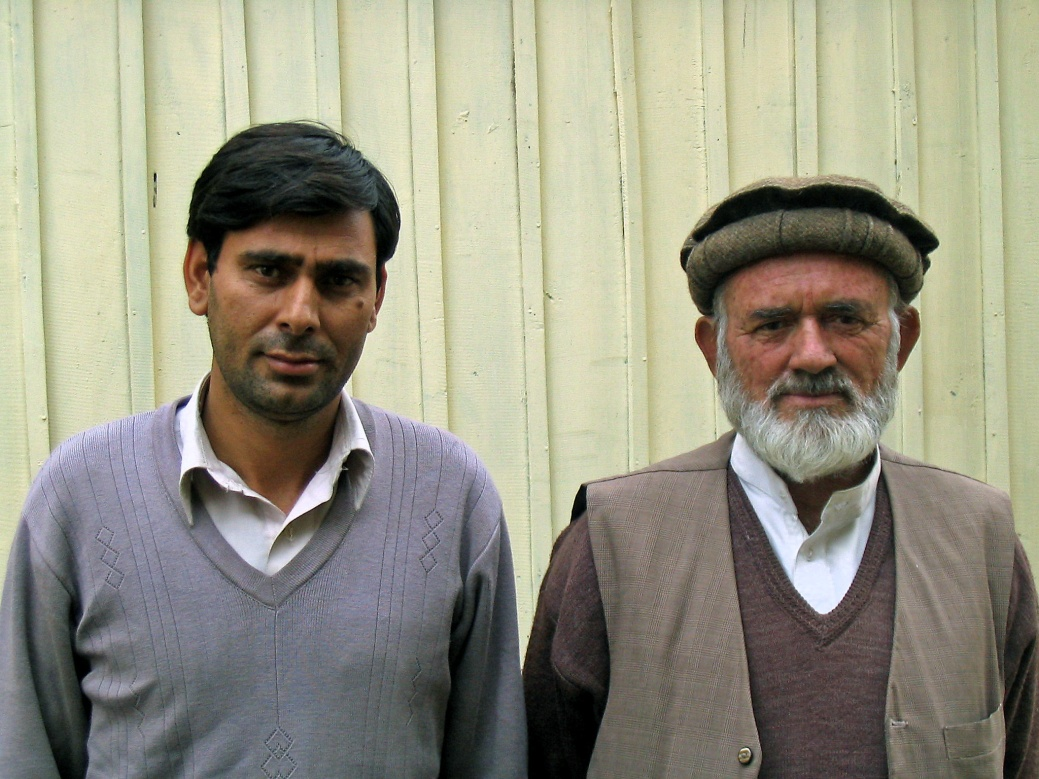
\includegraphics[width=\textwidth]{figures/ch1photo1.jpg}
\end{photofigure}

\textbf{Ikram ul"=Haq}, a~schoolteacher from Ashret, assisted me voluntarily in my research during
the period 1998--2000. He was introduced to transcription and basic recording methods and made
a~number of important interviews and text recordings, which he also transcribed and provided with
free translations.


\textbf{Sher Haider Khan}, a~schoolteacher from Ashret and older brother of Naseem Haider, assisted me
voluntarily on different occasions, filling in questionnaires, providing natural examples and
explaining various aspects of his language. He participated in parts of the FLI training programme.


A few other people spent considerable time with me, contributing in important ways to my research,
understanding and ability to speak Palula: Saeed Ahmad, Kalkatak; Atahullah, Biori; Sardar
Hayat, Ashret; (late) Said Habib, Ashret; Sher Habib, Ashret; and Munir Ahmad, Ashret.


My material on phonology is primarily based on separate B and A word lists\footnote{This included
  lexemes (primarily nouns and verbs) recorded in differently inflected forms as well as recordings
  of words in isolation and in frames.} that I began compiling and recording with speakers in
1999. Those have been supplemented later with other lists and recordings.


The morphological and syntactic parts of my study are primarily based on text material, in all 62
texts from 37 speakers/writers, of different length and analysed with varying accuracy and
detail. Most of the texts are recorded and transcribed oral narratives, but also other textual
genres are represented. A few texts in the material were written and in some cases only later
recorded when read out. However, even those written texts represent an~oral rather than a~literary
style, as there is no literary tradition. A tentative orthography was introduced as late as 2004,
and the written texts were produced during an~experimental phase in its development. The textual
material was supplemented with elicitation of full paradigms, local proverbs, expressions and sentences,
questionnaires and notes of language use in the community.


For details on textual genres, types of data and individual speakers and writers or informants, the
list in \textit{Abbreviations} at the beginning of this work should be consulted. The references given after
each example utterance throughout the work can be found in that list: for example, A:SHY028 refers to
a~particular narrative (abbreviated SHY) in the A variety (hence A:) written by Sher Haider, occurring as entry 28 in my interlinear text database.\footnote{A few texts are not entered as interlinear texts and therefore references to individual strings in them are not numbered.}


Although only marginally referred to and used, a~few smaller field studies carried out parallel with
my Palula research also need to be mentioned:


As already hinted at earlier, some \textbf{Sauji} data was collected in 2000, by Ajmal
Nuristani\footnote{Ajmal Nuristani's father is Nuristani and his mother's relatives come from Sau,
  but he is primarily a~Pashto speaker who grew up as a~refugee in Chitral.} and myself, in Timar
Camp in Lower Dir, where a~substantial number of people from Sau resided at the time. Later, Ajmal
Nuristani, at my request, recorded and transcribed a~few other texts and word lists, both in
Pakistan and in Sau (Afghanistan).


Also mentioned briefly above, a~survey trip to Kalkot in Dir Kohistan was carried out under Joan
Baart's (SIL) and my auspices by Naseem Haider and another FLI fellow, Muhammad Zaman Sagar (from
Kalam, Swat), in 2006. Apart from obtaining sociolinguistic information, they recorded a~few
\textbf{Kalkoti} texts, a~word list with two different speakers, a~questionnaire focusing on verbs
and another focusing on pronouns.


As for \textbf{Dameli}, data was chiefly collected in the form of a~questionnaire (dealing with
pronouns and verb agreement) filled out in the summer of 2005 by Muhammad Hayat Jan of Aspar (Damel
Valley), who participated in the FLI training program. The data was subsequently discussed with and
commented upon by Emil Perder (Stockholm University).\footnote{Emil Perder began field work on
  Dameli in 2003, through FLI, mainly with the aforementioned Muhammad Hayat and Asmat Ullah, also
  from Aspar, as co"=researchers and informants.}


Also in 2005, I carried out some interviews (based on the questionnaire also used for Dameli) in Kalkatak with Muhammad Salaam and Faiz Muhammad, two \textbf{Gawarbati} speakers, both in their thirties and originally from Nari in Afghanistan and since the early 1980s settled in the refugee section of the village Kalkatak.\footnote{I am indebted to my friend and FLI colleague Fakhruddin Akhunzada of Kalkatak for arranging these interviews.}


\section{Palula as a written language}
\label{sec:1-6b}

Until recently, Palula was unwritten and largely undocumented, a condition shared with most smaller (and even some larger) language communities in the region. Before the commencement of the current research, only a handful of local poets saw the need for writing Palula, making use of Urdu writing when composing poetry to be read aloud by themselves. There had been no systematic or collective attempts at creating a consistent and practical orthographic representation of Palula. The community is, after all, relatively small, with only a limited number of highly educated people, and uses a language entirely deprived of any outside recognition. Although there are primary schools throughout the Palula speaking area, only Urdu (and more recently English) is the recognised medium of instruction and formal literacy.


In 2003, representatives from all the major settlements came together and formed \textit{Anjuman-e-taraqqi-e-Palula}, a society for the promotion of Palula, with the purpose of facilitating the development of Palula as a vehicle for literary and educational efforts. At that time, an orthography proposal was put together by Naseem Haider and myself, with input from a few local scholars and teachers. It was endorsed by the society, which agreed that a Perso-Arabic script, conforming closely with the way it is applied to Urdu, should be used as a basis, with the addition of symbols representing a few consonant sounds not present in Urdu.\footnote{Words which are clearly identical to words in the Perso-Arabic stock are normally written in the traditional way, resulting in a fair degree of orthographic overrepresentation. The phoneme /s/ is, for example, represented by {\large\PRL{<س>}} in most native Palula vocabulary, but could be written as {\large\PRL{<س>}}, {\large\PRL{<ث>}} or {\large\PRL{<ص>}} if occurring in a loanword, depending on the particular spelling in the donor language.} The alphabet adopted is presented in \tabref{tab:1-4b}, displayed along with sound correspondences in the same broad transcription (``Palula Common Transcription'', or PCT) that is used throughout this work. Starting with a group of Urdu-literate people, the basic spelling principles were further discussed and applied in a writers’ workshop in 2004. Following some fine-tuning of the orthography, the two first-ever Palula booklets were printed in 2006, one of them an alphabet book \citep{haider2006a}\footnote{A second edition was published in 2012 \citep{haider2012a}.} and the other a collection of short stories \citep{haider2006b}. In 2012, Forum for Language Initiatives and Anjuman-e-taraqqi-e-Palula published a collection of about 300 Palula proverbs and sayings, along with Urdu translations \citep{haider2012b}.


Through the Forum for Language Initiatives, the concept of multilingual education was introduced to the community in 2005. This eventually led to the establishment of a mother-tongue pre-school in Ashret proper in 2008, and somewhat later a second school in Kooḍghaá. More than 30 native Palula speakers, both men and women, took part in producing the curricula from scratch, representing a set of culturally relevant themes. In preparation for the first school year, a package was produced consisting of a pre-reader, a pre-writer, a primer, a collection of reading stories, a collection of listening stories, and a compilation of songs and rhymes, all in Palula. In 2010, a first batch of pupils completed two years of education in Palula, with gradual introduction to Urdu and English \citep{rehmansagar2015}. 


\begin{table}
\caption{The Palula alphabet with corresponding transcription (PCT)}
\begin{tabularx}{\textwidth}{ Q Q Q Q Q Q Q }
\lsptoprule
\LARGE\PRL ج 
&\LARGE\PRL ث 
&\LARGE\PRL ٹ 
&\LARGE\PRL ت 
&\LARGE\PRL پ 
&\LARGE\PRL ب 
&\LARGE\PRL ا\\
\textit{ǰ} &
\textit{s} &
\textit{ṭ} &
\textit{t} &
\textit{p} &	
\textit{b} &	
\textit{a, aa}\\
\\
\LARGE\PRL ڈ
&\LARGE\PRL د 
&\LARGE\PRL خ 
&\LARGE\PRL ح 
&\LARGE\PRL څ 
&\LARGE\PRL ڇ 
&\LARGE\PRL چ\\
\textit{ḍ} &
\textit{d} &
\textit{x} &
\textit{h} &
\textit{ts} &	
\textit{c̣} &	
\textit{č}\\
\\
\LARGE\PRL س 
&\LARGE\PRL ڙ 
&\LARGE\PRL ژ 
&\LARGE\PRL ز 
&\LARGE\PRL ڑ 
&\LARGE\PRL ر 
&\LARGE\PRL ذ\\
\textit{s} &
\textit{ẓ} &
\textit{ǰ} &
\textit{z} &
\textit{ṛ} &	
\textit{r} &	
\textit{z}\\
\\
\LARGE\PRL ع 
&\LARGE\PRL ظ 
&\LARGE\PRL ط 
&\LARGE\PRL ض 
&\LARGE\PRL ص 
&\LARGE\PRL ݜ 
&\LARGE\PRL ش\\
\textit{-} &
\textit{z} &
\textit{t} &
\textit{z} &
\textit{s} &	
\textit{ṣ} &	
\textit{š}\\
\\
\LARGE\PRL م 
&\LARGE\PRL ل 
&\LARGE\PRL گ 
&\LARGE\PRL ک 
&\LARGE\PRL ق 
&\LARGE\PRL ف 
&\LARGE\PRL غ\\
\textit{m} &
\textit{l} &
\textit{ɡ} &
\textit{k} &
\textit{q} &	
\textit{f} &	
\textit{ɣ}\\
\\
\LARGE\PRL ے 
&\LARGE\PRL ی 
&\LARGE\PRL ھ 
&\LARGE\PRL ہ 
&\LARGE\PRL و 
&\LARGE\PRL ݨ 
&\LARGE\PRL ن\\
\textit{ee} &
\textit{y, ii} &
\textit{h} &
\textit{h} &
\textit{w, oo} &	
\textit{ṇ} &	
\textit{n}\\\lspbottomrule
\end{tabularx}
\label{tab:1-4b}
\end{table}


% Table X: The Palula alphabet with corresponding transcription
% ج	ث	ٹ	ت	پ	ب	ا
% ǰ	s	ṭ	t	p	b	a, aa
% ڈ	د	خ	ح	څ	ڇ	چ
% ḍ	d	x	h	ts	c̣	č
% س	ڙ	ژ	ز	ڑ	ر	ذ
% s	ẓ	ǰ	z	ṛ	r	z
% ع	ظ	ط	ض	ص	ڜ	ش
% -	z	t	z	s	ṣ	š
% م	ل	گ	ک	ق	ف	غ
% m	l	ɡ	k	q	f	ɣ
% ے 	ی	ھ	ہ	و	ڻ	ن
% ee	y, ii	h	h	w, oo	ṇ	n


The most visible modifications made to the existing Urdu alphabet in order to write Palula have to do with symbols representing a number of retroflex sounds: {\large\PRL{<ڇ>}}  for \textit{c̣}, {\large\PRL{<ڙ>}} for \textit{ẓ}, {\large\PRL{<ݜ>}} for \textit{ṣ}, and {\large\PRL{<ݨ>}} for \textit{ṇ}. To write \textit{ts}, the symbol {\large\PRL{<څ>}} has been borrowed from the Pashto alphabet. Aspiration as well as \textit{h} occurring in clusters with voiced consonants (see \tabref{tab:1-4bb}) are represented by {\large\PRL{<ھ>}}.


\begin{table}
\caption{Examples of Palula representation of ``aspiration''}
\begin{tabularx}{\textwidth}{ Q Q Q Q Q Q }
\lsptoprule
\LARGE\PRL{ پھ  }
&\LARGE\PRL{ تھ }
&\LARGE\PRL{ چھ }
&\LARGE\PRL{ دھ }
&\LARGE\PRL{ مھ }
&\LARGE\PRL{ بھر}\\
\textit{ph} &
\textit{th} &
\textit{čh} &
\textit{dh} &
\textit{mh} &
\textit{bhr}\\\lspbottomrule
\end{tabularx}
\label{tab:1-4bb}
\end{table}


Another modification relates to the representation of the ten vowels. Because of the many crucial contrasts between long and short vowels, particularly in word-final position, the developers of the Palula orthography introduced a language-particular use of a diacritic {\large\PRL{<ۡ>}} to mark a short vowel, as displayed in \tabref{tab:1-4c}. Mainly due to challenges in the area of font development, Palula materials are exclusively produced in naskh style, not in nasta’liq.


\begin{table}
\caption{Palula vowel representation}
\begin{tabularx}{\textwidth}{ Q Q Q Q Q }
\lsptoprule
\LARGE\PRL{{ اُو }}
&\LARGE\PRL{{ او }}
&\LARGE\PRL{{ ای }}
&\LARGE\PRL{{ اے }}
&\LARGE\PRL{{ آ}}\\
\textit{uu} &
\textit{oo} &
\textit{ii} &
\textit{ee} &
\textit{aa}\\
\\
\LARGE\PRL{{ اُ }}
&\LARGE\PRL{{ اوۡ }}
&\LARGE\PRL{{ اِ }}
&\LARGE\PRL{{ اےۡ }}
&\LARGE\PRL{{ ا }}\\
\textit{u} &
\textit{o} &
\textit{i} &
\textit{e} &
\textit{a}\\\lspbottomrule
\end{tabularx}
\label{tab:1-4c}
\end{table}


% Table Y: Palula vowel representation
% اُو	او	ای	اے	آ
% uu	oo	ii	ee	aa
% اُ	اوۡ	اِ	اےۡ	ا
% u	o	i	e	a


\section{Remarks on transcription and glossing}
\label{sec:1-7}

The trancription system used for Palula in the main bulk of this work (always occurring with
italics, for example, \textit{paaluulaá}) largely corresponds with that in general use in South Asian
linguistics and by most indologists (what \citeauthor{masica1991} refers to as ``Standard
Orientalist'', \citeyear[xv]{masica1991}, and some others refer to as an ``indological'' system,
\citealt[9]{radloff1999}). Since this is also the basic system (with very slight variations) used by other contemporary
scholars of Shina varieties
(\citealt{buddruss1987,buddruss1993,buddruss1996,degener2008,schmidtkohistani2001,schmidtkohistani2008,schmidt2000,schmidt2001,schmidt2003,schmidt2004,schmidt2004b, radloff1992,radloff1999};
{Radloff w. Shakil \citeyear{radloffshakil1998})\footnote{Also the transcriptions in
    \citet{hook1990a,hook1996} and \citet{hookzia2005} agree to a~large extent with the principles
    applied by the other scholars.}, including the conventions for representing accent (for details,
  see \sectref{subsec:3-4-3}), I have seen no reason to abandon it in favour of any other standard, such as
  a~consistent use of IPA symbols, since any such decision would make inter"=variety comparisons more
  troublesome and less straight"=forward. I will, as mentioned (\sectref{sec:1-6b}), refer to this broad transcription, taking only phonological contrasts into account, as \textit{Palula common transcription} (PCT). The PCT symbols that differ from IPA notation are listed in \tabref{tab:1-5}.


However, to make the work accessible to the general typologist or readers not familiar with this
particular system, IPA transcription (following International Phonetic Association, 1999) has been
used (along with PCT within parentheses) for phonemic and phonetic
transcriptions in \sectref{sec:3-1}--\sectref{sec:3-4} (and occasionally elsewhere in the grammar), the former consistently surrounded by forward slashes, for example /paːluːlǎː/, and the latter by square brackets, for example [paːɫuːɫǎː]. 


When citing other sources or scholars on individual IA languages, I have in most cases kept the
transcription used by them, without any attempts at making them conform to the particular
conventions used in Palula examples.


\begin{table}[ht]
\caption{Symbols used in Palula common transcription (PCT) deviating from IPA notation}
\begin{tabularx}{.8\textwidth}{ l l   Q }
\lsptoprule
PCT &
IPA &
Comment\\\midrule
\textit{ṭ} &
ʈ &
\\
\textit{ḍ} &
ɖ &
\\
\textit{c̣} &
ʈʂ &
\\
\textit{č} &
ʨ &
\\
\textit{ṣ} &
ʂ &
\\
\textit{š} &
ɕ &
\\
\textit{ẓ} &
ʐ &
\\
\textit{ǰ} &
ʑ &\\


\textit{ṇ} &
ɳ &
\\
\textit{ṛ} &
ɽ &
\\
\textit{y} &
j &
\\
\textit{h} &
ʰ &
Aspiration (h following voiceless plosive or affricate in PCT)
\\
\textit{aa} &
aː &
Double vowel corr. to IPA length"=indicating /ː/
\\
\textit{áa} &
âː &
First"=mora accent
\\
\textit{aá} &
ǎː &
Second"=mora accent
\\
\textit{a}\textasciitilde &
ã &
Nasalisation\\\lspbottomrule
\end{tabularx}
\label{tab:1-5}
\end{table}

I should hasten to add that PCT is not to be considered a~community
orthography. For that purpose the Arabic"=based script (as described in \sectref{sec:1-6b}) is used and promoted in the community.


Each glossed example sentence in this work consists (with a few exceptions) of three lines or analytical strings: 1) A transcribed utterance, 2) morpheme glossing, and 3) a free translation. The first line is a phonemic representation of the utterance, following PTC (as described above), with word breaks and morpheme breaks. It is, as far as has been possible, a regularised (within each of the two main dialects) surface form, i.e., a form not necessarily reflecting underlying morphology nor individual sub-phonemic variation. Some deviations from these principles have been applied when there is considerable (intra"=dialectal) variation in the output form, such as in the representation of the present tense suffix \textit{-áan} when following on an \textit{a}"=ending stem. In most cases, however, morpheme breaks (e.g., \textit{phed-í} `arrive"=\textsc{cv}') have only been applied (i.e., signalled explicitly with a hyphen) when they line up with the surface form, whereas  sequences of morphemic elements obscured by the surface form (e.g., \textit{seé} `sleep.\textsc{cv}') are only separated with a period in the glossing while represented as a single element in the transcription itself. On the second line, each morpheme is shown with a gloss, either in the form of a one"=word English equivalent of a lexical morpheme, or in the form of an abbreviation of a grammatical category. The third line gives a free translation into English of the utterance as a whole; it strives at capturing the meaning in idiomatic English.


Slightly different principles have been applied to the two sample texts included. Instead of the three analytical strings of the glossed examples, there are four separate strings: 1) A transcribed utterance, 2) morpheme breakdown, 3) morpheme glossing, and 4) a free translation. The first line, again reflecting a regularised surface form, is only given with word breaks, no word"=internal morpheme breaks. The second line has the transcribed Palula words broken down into morphemes. These are, to the extent it has been possible, displayed in an underlying morphemic form, which in some cases differ slightly from the output form of the first line. The third line, that of morpheme glossing, lines up with the morpheme breakdown of the second line. Frequently occurring markers have in this version been supplied with more specific glossing. The same principles as above have been applied to the free translation. 

%% OLD
%% \begin{table}[ht]
%% \label{bkm:Ref193267319}
%% \caption{Symbols used in Palula common transcription (PCT) deviating from IPA notation}
%% \begin{tabularx}{\textwidth}{ l l | l l Q }
%% \lsptoprule
%% PCT &
%% IPA &
%% PCT &
%% IPA &
%% Comment\\\midrule
%% \textit{ṭ} &
%% ʈ &
%% \textit{ṇ} &
%% ɳ &
%% \\
%% \textit{ḍ} &
%% ɖ &
%% \textit{ṛ} &
%% ɽ &
%% \\
%% \textit{c̣} &
%% ʈʂ &
%% \textit{y} &
%% j &
%% \\
%% \textit{č} &
%% ʨ &
%% \textit{h} &
%% ʰ &
%% Aspiration (h following C in PCT)\\
%% \textit{ṣ} &
%% ʂ &
%% \textit{aa} &
%% aː &
%% Double vowel corr. to IPA length"=indicating /ː/\\
%% \textit{š} &
%% ɕ &
%% \textit{áa} &
%% âː &
%% First"=mora accent\\
%% \textit{ẓ} &
%% ʐ &
%% \textit{aá} &
%% ǎː &
%% Second"=mora accent\\
%% \textit{ǰ} &
%% ʑ &
%% \textit{ã} &
%% ã &
%% Nasalisation\\\lspbottomrule
%% \end{tabularx}
%% \label{tab:1-5}
%% \end{table}